% Autor: Jose Ricardo Bustos Molina
%        Universidad del Tolima
%        jrbustosm@ut.edu.co
%

%--------------------------------------------------------------------------------
%Definición función para graficar cartas
%--------------------------------------------------------------------------------
\definecolor{mygray}{RGB}{200,200,200}
\definecolor{mydarkgray}{RGB}{30,30,30}
\pgfSetupImageAsPattern[width=15cm]{marble}{img/marbel.jpg}
\pgfSetupImageAsPattern[width=15cm]{verde}{img/verde.jpg}
\pgfSetupImageAsPattern[width=15cm]{azul}{img/azul.jpg}
\pgfSetupImageAsPattern[width=15cm]{morado}{img/morado.jpg}
% Keys for rectangle with inverted corners
%
% /pgf/rectangle with inverted corners selected : specify the corners to invert.
% /pgf/rectangle with inverted corners radius   : set the radius of the corners.

\makeatletter
\pgfkeys{/pgf/rectangle with inverted corners selected/.store in=\pgf@lib@sh@misc@convrect@corners}
\pgfkeys{/tikz/rectangle with inverted corners selected/.store in=\pgf@lib@sh@misc@convrect@corners}

\def\pgf@lib@sh@misc@convrect@invertall{invert all}%
\def\pgf@lib@sh@misc@convrect@invert{invert}
\let\pgf@lib@sh@misc@convrect@corners\pgf@lib@sh@misc@convrect@invertall


\def\pgf@lib@sh@misc@convrect@getcorners{%
  \let\northeastcorner\pgfutil@empty%
  \let\southeastcorner\pgfutil@empty%
  \let\southwestcorner\pgfutil@empty%
  \let\northwestcorner\pgfutil@empty%
  \expandafter\pgfutil@in@\expandafter{\pgf@lib@sh@misc@convrect@corners}{invert all}%
  \ifpgfutil@in@%
    \let\northeastcorner\pgf@lib@sh@misc@convrect@invert%
    \let\southeastcorner\pgf@lib@sh@misc@convrect@invert%
    \let\southwestcorner\pgf@lib@sh@misc@convrect@invert%
    \let\northwestcorner\pgf@lib@sh@misc@convrect@invert%
    \let\pgf@next\relax%
  \else%
    \let\pgf@next\pgf@lib@sh@misc@convrect@parsecorners%
  \fi%
  \pgf@next}

\def\pgf@lib@sh@misc@convrect@parsecorners{%
  \expandafter\pgf@@concaverectangle@parsecorners\pgf@lib@sh@misc@convrect@corners,\pgf@stop,%
}

\def\pgf@@concaverectangle@parsecorners#1,{%
  \ifx#1\pgf@stop%
    \let\pgf@next\relax%
  \else%
    \pgfutil@in@{@#1@}{@north east@@top left@}%
    \ifpgfutil@in@%
      \let\northeastcorner\pgf@lib@sh@misc@convrect@invert%
    \else%
      \pgfutil@in@{@#1@}{@south east@@bottom right@}%
      \ifpgfutil@in@%
        \let\southeastcorner\pgf@lib@sh@misc@convrect@invert%
      \else%
        \pgfutil@in@{@#1@}{@south west@@bottom left@}%
        \ifpgfutil@in@%
          \let\southwestcorner\pgf@lib@sh@misc@convrect@invert%
        \else%
          \pgfutil@in@{@#1@}{@north west@@top right@}%
          \ifpgfutil@in@%
            \let\northwestcorner\pgf@lib@sh@misc@convrect@invert%
          \fi%
        \fi%
      \fi%
    \fi%
    \let\pgf@next\pgf@@@concaverectangle@parsecorners%
  \fi%
  \pgf@next%
}
\def\pgf@@@concaverectangle@parsecorners{%
  \pgfutil@ifnextchar x{\pgf@@concaverectangle@parsecorners}{\pgf@@concaverectangle@parsecorners}%
}%

\pgfkeys{/pgf/.cd,
  rectangle with inverted corners radius/.initial=.666ex%
}




% Shape rectangle with inverted corners.
%
%
\pgfdeclareshape{rectangle with inverted corners}{%
  \savedmacro\getconcaverectanglepoints{%
    \pgf@lib@sh@misc@convrect@getcorners%
    %
    % Get the node dimensions.
    %
    \pgfmathsetlength\pgf@xa{\pgfkeysvalueof{/pgf/inner xsep}}%
    \advance\pgf@xa.5\wd\pgfnodeparttextbox%
    \pgfmathsetlength\pgf@ya{\pgfkeysvalueof{/pgf/inner ysep}}%
    \advance\pgf@ya.5\ht\pgfnodeparttextbox%
    \advance\pgf@ya.5\dp\pgfnodeparttextbox%
    %
    % Get invert stuff.
    %
    \pgfmathsetlengthmacro\convsep{\pgfkeysvalueof{/pgf/rectangle with inverted corners radius}}%
    \pgfmathsetlength\pgf@xc{\convsep/sqrt(2)}%
    \pgfmathsetlength\pgf@yc{\convsep/sqrt(2)}%
    \addtosavedmacro\convsep%
    %
    % Check for minimum width and height%
    %
    \pgfutil@tempdima\pgf@xa%
    \advance\pgfutil@tempdima\convsep%
    \pgfmathsetlength\pgfutil@tempdimb{\pgfkeysvalueof{/pgf/minimum width}}%
    \ifdim\pgfutil@tempdima<.5\pgfutil@tempdimb%
      \pgf@xa.5\pgfutil@tempdimb%
    \fi%
    \pgfutil@tempdima\pgf@ya%
    \advance\pgfutil@tempdima\convsep%
    \pgfmathsetlength\pgfutil@tempdimb{\pgfkeysvalueof{/pgf/minimum height}}%
    \ifdim\pgfutil@tempdima<.5\pgfutil@tempdimb%
      \pgf@ya.5\pgfutil@tempdimb%
    \fi%
    %
    % Define the background path points.
    %
    \pgfextract@process\centerpoint{%
      \pgfmathsetlength\pgf@x{+.5\wd\pgfnodeparttextbox}%
      \pgfmathsetlength\pgf@y{+.5\ht\pgfnodeparttextbox}%
      \pgfmathaddtolength\pgf@y{+-.5\dp\pgfnodeparttextbox}%
    }%
    \pgfextract@process\beforenortheast{%
      \centerpoint%
      \advance\pgf@x\pgf@xa%
      \advance\pgf@y\pgf@ya%
      \advance\pgf@y-\convsep%
    }%
    \pgfextract@process\northeast{%
      \centerpoint%
      \advance\pgf@x\pgf@xa%
      \advance\pgf@y\pgf@ya%
      \ifx\northeastcorner\pgfutil@empty%
      \else
        \advance\pgf@x-\pgf@xc%
        \advance\pgf@y-\pgf@yc%
      \fi%
    }%
    \pgfextract@process\afternortheast{%
      \centerpoint%
      \advance\pgf@x\pgf@xa%
      \advance\pgf@x-\convsep%
      \advance\pgf@y\pgf@ya%
    }%
    \pgfextract@process\beforenorthwest{%
      \centerpoint%
      \advance\pgf@x-\pgf@xa%
      \advance\pgf@x\convsep%
      \advance\pgf@y\pgf@ya%
    }%
    \pgfextract@process\northwest{%
      \centerpoint%
      \advance\pgf@x-\pgf@xa%
      \advance\pgf@y\pgf@ya%
      \ifx\northwestcorner\pgfutil@empty%
      \else
        \advance\pgf@x\pgf@xc%
        \advance\pgf@y-\pgf@yc%
      \fi%
    }%
    \pgfextract@process\afternorthwest{%
      \centerpoint%
      \advance\pgf@x-\pgf@xa%
      \advance\pgf@y\pgf@ya%
      \advance\pgf@y-\convsep%
    }%
    \pgfextract@process\beforesouthwest{%
      \centerpoint%
      \advance\pgf@x-\pgf@xa%
      \advance\pgf@y-\pgf@ya%
      \advance\pgf@y\convsep%
    }%
    \pgfextract@process\southwest{%
      \centerpoint%
      \advance\pgf@x-\pgf@xa%
      \advance\pgf@y-\pgf@ya%
      \ifx\southwestcorner\pgfutil@empty%
      \else
        \advance\pgf@x\pgf@xc%
        \advance\pgf@y\pgf@yc%
      \fi%
    }%
    \pgfextract@process\aftersouthwest{%
      \centerpoint%
      \advance\pgf@x-\pgf@xa%
      \advance\pgf@x\convsep%
      \advance\pgf@y-\pgf@ya%
    }%
    \pgfextract@process\beforesoutheast{%
      \centerpoint%
      \advance\pgf@x\pgf@xa%
      \advance\pgf@x-\convsep%
      \advance\pgf@y-\pgf@ya%
    }%
    \pgfextract@process\southeast{%
      \centerpoint%
      \advance\pgf@x\pgf@xa%
      \advance\pgf@y-\pgf@ya%
      \ifx\southeastcorner\pgfutil@empty%
      \else
        \advance\pgf@x-\pgf@xc%
        \advance\pgf@y\pgf@yc%
      \fi%
    }%
    \pgfextract@process\aftersoutheast{%
      \centerpoint%
      \advance\pgf@x\pgf@xa%
      \advance\pgf@y-\pgf@ya%
      \advance\pgf@y\convsep%
    }%
    \addtosavedmacro\beforenortheast%
    \addtosavedmacro\afternortheast%
    \addtosavedmacro\beforesouthwest%
    \addtosavedmacro\aftersouthwest%
    %
    % Calculate the `miter' vectors.
    %
    \pgfmathsetlengthmacro\outerxsep{\pgfkeysvalueof{/pgf/outer xsep}}%
    \pgfmathsetlengthmacro\outerysep{\pgfkeysvalueof{/pgf/outer ysep}}%
    \addtosavedmacro\outerxsep%
    \addtosavedmacro\outerysep%
    \pgfextract@process\before@ne@anchor{%
      \beforenortheast%
      \advance\pgf@x\outerxsep%
      \advance\pgf@y\outerysep%
    }%
    \pgfextract@process\before@sw@anchor{%
      \beforesouthwest%
      \advance\pgf@x-\outerxsep%
      \advance\pgf@y-\outerysep%
    }%
    \pgfextract@process\after@ne@anchor{%
      \afternortheast%
      \advance\pgf@x\outerxsep%
      \advance\pgf@y\outerysep%
    }%
    \pgfextract@process\after@sw@anchor{%
      \aftersouthwest
      \advance\pgf@x-\outerxsep%
      \advance\pgf@y-\outerysep%
    }%
    \addtosavedmacro\before@ne@anchor%
    \addtosavedmacro\after@ne@anchor%
    \addtosavedmacro\before@sw@anchor%
    \addtosavedmacro\after@sw@anchor%
    \pgfextract@process\ne@anchor{%
      \northeast%
      \ifx\northeastcorner\pgfutil@empty%
        \pgfmathaddtolength\pgf@x{\pgfkeysvalueof{/pgf/outer xsep}}%
        \pgfmathaddtolength\pgf@y{\pgfkeysvalueof{/pgf/outer ysep}}%
      \else%
        \pgfmathaddtolength\pgf@x{\pgfkeysvalueof{/pgf/outer xsep}/sqrt(2)}%
        \pgfmathaddtolength\pgf@y{\pgfkeysvalueof{/pgf/outer ysep}/sqrt(2)}%
      \fi%
    }%
    \pgfextract@process\nw@anchor{%
      \northwest%
      \ifx\northwestcorner\pgfutil@empty%
        \pgfmathaddtolength\pgf@x{-\pgfkeysvalueof{/pgf/outer xsep}}%
        \pgfmathaddtolength\pgf@y{\pgfkeysvalueof{/pgf/outer ysep}}%
      \else%
        \pgfmathaddtolength\pgf@x{-\pgfkeysvalueof{/pgf/outer xsep}/sqrt(2)}%
        \pgfmathaddtolength\pgf@y{\pgfkeysvalueof{/pgf/outer ysep}/sqrt(2)}%
      \fi%
    }%
    \pgfextract@process\sw@anchor{%
      \southwest%
      \ifx\southwestcorner\pgfutil@empty%
        \pgfmathaddtolength\pgf@x{-\pgfkeysvalueof{/pgf/outer xsep}}%
        \pgfmathaddtolength\pgf@y{-\pgfkeysvalueof{/pgf/outer ysep}}%
      \else%
        \pgfmathaddtolength\pgf@x{-\pgfkeysvalueof{/pgf/outer xsep}/sqrt(2)}%
        \pgfmathaddtolength\pgf@y{-\pgfkeysvalueof{/pgf/outer ysep}/sqrt(2)}%
      \fi%
    }%
    \pgfextract@process\se@anchor{%
      \southeast%
      \ifx\southeastcorner\pgfutil@empty%
        \pgfmathaddtolength\pgf@x{\pgfkeysvalueof{/pgf/outer xsep}}%
        \pgfmathaddtolength\pgf@y{-\pgfkeysvalueof{/pgf/outer ysep}}%
      \else%
        \pgfmathaddtolength\pgf@x{\pgfkeysvalueof{/pgf/outer xsep}/sqrt(2)}%
        \pgfmathaddtolength\pgf@y{-\pgfkeysvalueof{/pgf/outer ysep}/sqrt(2)}%
      \fi%
    }%
    \addtosavedmacro\ne@anchor%
    \addtosavedmacro\nw@anchor%
    \addtosavedmacro\sw@anchor%
    \addtosavedmacro\se@anchor%
    \addtosavedmacro\northwestcorner
    \addtosavedmacro\northeastcorner
    \addtosavedmacro\southwestcorner
    \addtosavedmacro\southeastcorner
  }%
  \savedanchor\centerpoint{%
    \pgf@x.5\wd\pgfnodeparttextbox%
    \pgf@y.5\ht\pgfnodeparttextbox%
    \advance\pgf@y-.5\dp\pgfnodeparttextbox%
  }%
  \savedanchor\midpoint{%
    \pgf@x.5\wd\pgfnodeparttextbox%
    \pgfmathsetlength\pgf@y{+.5ex}%
  }%
  \savedanchor\basepoint{%
    \pgf@x.5\wd\pgfnodeparttextbox%
    \pgf@y0pt%
  }%
  \anchor{center}{\centerpoint}%
  \anchor{mid}{\midpoint}%
  \anchor{mid east}{%
    \getconcaverectanglepoints%
    \midpoint%
    \pgf@ya\pgf@y%
    \pgf@process{%
      \before@sw@anchor%
      \pgf@ya\pgf@y%
      \before@ne@anchor%
      \pgf@y\pgf@ya
    }%
    \ifdim\pgf@ya<\pgf@y%
      \pgfpointintersectionoflines{\midpoint}{\midpoint\pgf@ya\pgf@y\before@ne@anchor\pgf@y\pgf@ya}%
        {\before@sw@anchor\pgf@ya\pgf@y\before@ne@anchor\pgf@y\pgf@ya}%
        {\after@sw@anchor\pgf@ya\pgf@y\after@ne@anchor\pgf@y\pgf@ya}%
    \else%
      \pgf@process{\before@ne@anchor}%
      \ifdim\pgf@ya<\pgf@y%
        \pgfpointintersectionoflines{\midpoint}{\midpoint\pgf@ya\pgf@y\before@ne@anchor\pgf@y\pgf@ya}%
          {\before@sw@anchor\pgf@ya\pgf@y\before@ne@anchor\pgf@y\pgf@ya}%
          {\before@ne@anchor}%
      \else%
        \pgfpointintersectionoflines{\midpoint}{\midpoint\pgf@ya\pgf@y\before@ne@anchor\pgf@y\pgf@ya}%
          {\before@ne@anchor}%
          {\after@ne@anchor}%
      \fi%
    \fi%
  }%
  \anchor{mid west}{%
    \getconcaverectanglepoints%
    \midpoint%
    \pgf@ya\pgf@y%
    \pgf@process{\before@sw@anchor}%
    \ifdim\pgf@ya<\pgf@y%
      \pgfpointintersectionoflines{\midpoint}{\midpoint\pgf@ya\pgf@y\before@sw@anchor\pgf@y\pgf@ya}%
        {\before@sw@anchor}{\after@sw@anchor}%
    \else%
      \pgf@process{\before@ne@anchor\pgf@ya\pgf@y\before@sw@anchor\pgf@y\pgf@ya}%
      \ifdim\pgf@ya<\pgf@y%
        \pgfpointintersectionoflines{\midpoint}{\midpoint\pgf@ya\pgf@y\before@sw@anchor\pgf@y\pgf@ya}%
          {\before@ne@anchor\pgf@ya\pgf@y\before@sw@anchor\pgf@y\pgf@ya}%
          {\before@sw@anchor}%
      \else%
        \pgfpointintersectionoflines{\midpoint}{\midpoint\pgf@ya\pgf@y\before@sw@anchor\pgf@y\pgf@ya}%
          {\before@ne@anchor\pgf@ya\pgf@y\before@sw@anchor\pgf@y\pgf@ya}%
          {\after@ne@anchor\pgf@ya\pgf@y\after@sw@anchor\pgf@y\pgf@ya}%
      \fi%
    \fi%
  }%
  \anchor{base}{\basepoint}%
  \anchor{base east}{%
    \getconcaverectanglepoints%
    \basepoint%
    \pgf@ya\pgf@y%
    \pgf@process{%
      \before@sw@anchor%
      \pgf@ya\pgf@y%
      \before@ne@anchor%
      \pgf@y\pgf@ya
    }%
    \ifdim\pgf@ya<\pgf@y%
      \pgfpointintersectionoflines{\basepoint}{\basepoint\pgf@ya\pgf@y\before@ne@anchor\pgf@y\pgf@ya}%
        {\before@sw@anchor\pgf@ya\pgf@y\before@ne@anchor\pgf@y\pgf@ya}%
        {\after@sw@anchor\pgf@ya\pgf@y\after@ne@anchor\pgf@y\pgf@ya}%
    \else%
      \pgf@process{\before@ne@anchor}%
      \ifdim\pgf@ya<\pgf@y%
        \pgfpointintersectionoflines{\basepoint}{\basepoint\pgf@ya\pgf@y\before@ne@anchor\pgf@y\pgf@ya}%
          {\before@sw@anchor\pgf@ya\pgf@y\before@ne@anchor\pgf@y\pgf@ya}%
          {\before@ne@anchor}%
      \else%
        \pgfpointintersectionoflines{\basepoint}{\basepoint\pgf@ya\pgf@y\before@ne@anchor\pgf@y\pgf@ya}%
          {\before@ne@anchor}%
          {\after@ne@anchor}%
      \fi%
    \fi%
  }%
  \anchor{base west}{%
    \getconcaverectanglepoints%
    \basepoint%
    \pgf@ya\pgf@y%
    \pgf@process{\before@sw@anchor}%
    \ifdim\pgf@ya<\pgf@y%
      \pgfpointintersectionoflines{\basepoint}{\basepoint\pgf@ya\pgf@y\before@sw@anchor\pgf@y\pgf@ya}%
        {\before@sw@anchor}{\after@sw@anchor}%
    \else%
      \pgf@process{\before@ne@anchor\pgf@ya\pgf@y\before@sw@anchor\pgf@y\pgf@ya}%
      \ifdim\pgf@ya<\pgf@y%
        \pgfpointintersectionoflines{\basepoint}{\basepoint\pgf@ya\pgf@y\before@sw@anchor\pgf@y\pgf@ya}%
          {\before@ne@anchor\pgf@ya\pgf@y\before@sw@anchor\pgf@y\pgf@ya}%
          {\before@sw@anchor}%
      \else%
        \pgfpointintersectionoflines{\basepoint}{\basepoint\pgf@ya\pgf@y\before@sw@anchor\pgf@y\pgf@ya}%
          {\before@ne@anchor\pgf@ya\pgf@y\before@sw@anchor\pgf@y\pgf@ya}%
          {\after@ne@anchor\pgf@ya\pgf@y\after@sw@anchor\pgf@y\pgf@ya}%
      \fi%
    \fi%
  }%
  \anchor{before north east}{\getconcaverectanglepoints\before@ne@anchor}%
  \anchor{north east}{\getconcaverectanglepoints\ne@anchor}%
  \anchor{after north east}{\getconcaverectanglepoints\after@ne@anchor}%
  \anchor{north}{%
    \getconcaverectanglepoints%
    \centerpoint%
    \pgf@xa\pgf@x%
    \after@ne@anchor%
    \pgf@x\pgf@xa}%
  \anchor{before north west}{%
    \getconcaverectanglepoints%
    \after@sw@anchor%
    \pgf@xa\pgf@x%
    \after@ne@anchor%
    \pgf@x\pgf@xa}%
  \anchor{north west}{\getconcaverectanglepoints\nw@anchor}%
  \anchor{after north west}{%
    \getconcaverectanglepoints%
    \before@sw@anchor%
    \pgf@xa\pgf@x%
    \before@ne@anchor%
    \pgf@x\pgf@xa}%
  \anchor{west}{%
    \getconcaverectanglepoints%
    \centerpoint%
    \pgf@ya\pgf@y%
    \before@sw@anchor%
    \pgf@y\pgf@ya}%
  \anchor{before south west}{\getconcaverectanglepoints\before@sw@anchor}%
  \anchor{south west}{\getconcaverectanglepoints\sw@anchor}%
  \anchor{after south west}{\getconcaverectanglepoints\after@sw@anchor}%
    \anchor{south}{%
    \getconcaverectanglepoints%
    \centerpoint%
    \pgf@xa\pgf@x%
    \after@sw@anchor%
    \pgf@x\pgf@xa}%
  \anchor{before south east}{%
    \getconcaverectanglepoints%
    \after@sw@anchor%
    \pgf@ya\pgf@y%
    \after@ne@anchor%
    \pgf@y\pgf@ya}%
  \anchor{south east}{\getconcaverectanglepoints\se@anchor}%
  \anchor{after south east}{%
    \getconcaverectanglepoints%
    \before@sw@anchor%
    \pgf@ya\pgf@y%
    \before@ne@anchor%
    \pgf@y\pgf@ya}%
  \anchor{east}{%
    \getconcaverectanglepoints%
    \centerpoint%
    \pgf@ya\pgf@y%
    \before@ne@anchor%
    \pgf@y\pgf@ya}%
  \backgroundpath{%
    \pgfpathmoveto{\beforenortheast}%
    \ifx\northeastcorner\pgfutil@empty%
      \pgfpathlineto{\northeast}%
    \else%
      \pgfpatharc{-90}{-180}{\convsep}%
    \fi%
    \pgfpathlineto{\beforenorthwest}%
    \ifx\northwestcorner\pgfutil@empty%
      \pgfpathlineto{\northwest}%
    \else%
      \pgfpatharc{0}{-90}{\convsep}%
    \fi%
    \pgfpathlineto{\beforesouthwest}%
    \ifx\southwestcorner\pgfutil@empty%
      \pgfpathlineto{\southwest}%
    \else%
      \pgfpatharc{90}{0}{\convsep}%
    \fi%
    \pgfpathlineto{\beforesoutheast}%
    \ifx\southeastcorner\pgfutil@empty%
      \pgfpathlineto{\southeast}%
    \else%
      \pgfpatharc{180}{90}{\convsep}%
    \fi%
    \pgfpathclose%
    %
  }
  \anchorborder{%
    \pgfextract@process\externalpoint{%
      \pgf@xa\pgf@x%
      \pgf@ya\pgf@y%
      \centerpoint%
      \advance\pgf@x\pgf@xa%
      \advance\pgf@y\pgf@ya%
    }%
    \pgfmathanglebetweenpoints{\centerpoint}{\externalpoint}%
    \let\externalangle\pgfmathresult%
    \getconcaverectanglepoints%
    \pgfmathanglebetweenpoints{\centerpoint}{\before@ne@anchor\pgf@xa\pgf@x\before@sw@anchor\pgf@x\pgf@xa}%
    \ifdim\externalangle pt<\pgfmathresult pt\relax% < after south east.
      \pgfmathanglebetweenpoints{\centerpoint}{\after@ne@anchor\pgf@xa\pgf@x\after@sw@anchor\pgf@x\pgf@xa}%
      \ifdim\externalangle pt<\pgfmathresult pt\relax% < before south east.
        \pgfmathanglebetweenpoints{\centerpoint}{\after@sw@anchor}%
        \ifdim\externalangle pt<\pgfmathresult pt\relax% < after south west.
          \pgfmathanglebetweenpoints{\centerpoint}{\before@sw@anchor}%
          \ifdim\externalangle pt<\pgfmathresult pt\relax% < before south west.
            \pgfmathanglebetweenpoints{\centerpoint}{\before@sw@anchor\pgf@xa\pgf@x\before@ne@anchor\pgf@x\pgf@xa}%
            \ifdim\externalangle pt<\pgfmathresult pt\relax% < after north west.
              \pgfmathanglebetweenpoints{\centerpoint}{\after@sw@anchor\pgf@xa\pgf@x\after@ne@anchor\pgf@x\pgf@xa}%
              \ifdim\externalangle pt<\pgfmathresult pt\relax% < before north west.
                \pgfmathanglebetweenpoints{\centerpoint}{\after@ne@anchor}%
                \ifdim\externalangle pt<\pgfmathresult pt\relax% < after north east.
                  \pgfmathanglebetweenpoints{\centerpoint}{\before@ne@anchor}%
                  \ifdim\externalangle pt<\pgfmathresult pt\relax% < before north east.
                    % east side (> 0°)
                    \pgfpointintersectionoflines{\centerpoint}{\externalpoint}%
                      {\before@ne@anchor\pgf@xa\pgf@x\before@sw@anchor\pgf@x\pgf@xa}{\before@ne@anchor}%
                  \else%
                    % top right corner
                    \ifx\northeastcorner\pgfutil@empty\relax%
                      % rectangle corner
                      \pgfmathanglebetweenpoints{\centerpoint}{\ne@anchor}%
                      \ifdim\externalangle pt<\pgfmathresult pt\relax% < north east.
                        % intersect with east side
                        \pgfpointintersectionoflines{\centerpoint}{\externalpoint}%
                          {\before@ne@anchor\pgf@xa\pgf@x\before@sw@anchor\pgf@x\pgf@xa}{\before@ne@anchor}%
                      \else% > north west
                        % intersect with north side
                        \pgfpointintersectionoflines{\centerpoint}{\externalpoint}%
                          {\after@ne@anchor}{\after@sw@anchor\pgf@xa\pgf@x\after@ne@anchor\pgf@x\pgf@xa}%
                      \fi%
                    \else%
                      % inverted corner
                      \pgfextract@process\arccenter{%
                        \beforenortheast%
                        \pgf@xa\pgf@x%
                        \afternortheast%
                        \pgf@x\pgf@xa%
                      }%
                      \pgfmathpointintersectionoflineandarc{\externalpoint}{\centerpoint}%
                        {\arccenter}{-80}{-190}{\convsep-\outerxsep and \convsep-\outerysep}%
                    \fi%
                  \fi%
                \else%
                  % north side
                  \pgfpointintersectionoflines{\centerpoint}{\externalpoint}%
                    {\after@ne@anchor}{\after@sw@anchor\pgf@xa\pgf@x\after@ne@anchor\pgf@x\pgf@xa}%
                \fi%
              \else%
                % top left corner
                \ifx\northwestcorner\pgfutil@empty\relax%
                  % rectangle corner
                  \pgfmathanglebetweenpoints{\centerpoint}{\nw@anchor}%
                  \ifdim\externalangle pt<\pgfmathresult pt\relax% < north west.
                    % intersect with north side
                    \pgfpointintersectionoflines{\centerpoint}{\externalpoint}%
                      {\after@ne@anchor}{\after@sw@anchor\pgf@xa\pgf@x\after@ne@anchor\pgf@x\pgf@xa}%
                  \else% > north west
                    % intersect with west side
                    \pgfpointintersectionoflines{\centerpoint}{\externalpoint}%
                      {\before@sw@anchor\pgf@xa\pgf@x\before@ne@anchor\pgf@x\pgf@xa}{\before@sw@anchor}%
                  \fi%
                \else%
                  % inverted corner
                  \pgfextract@process\arccenter{%
                    \beforesouthwest%
                    \pgf@xa\pgf@x%
                    \afternortheast%
                    \pgf@x\pgf@xa%
                  }%
                  \pgfmathpointintersectionoflineandarc{\externalpoint}{\centerpoint}%
                    {\arccenter}{10}{-100}{\convsep-\outerxsep and \convsep-\outerysep}%
                \fi%
              \fi%
            \else%
              % west side
              \pgfpointintersectionoflines{\centerpoint}{\externalpoint}%
                {\before@sw@anchor\pgf@xa\pgf@x\before@ne@anchor\pgf@x\pgf@xa}{\before@sw@anchor}%
            \fi%
          \else%
            % bottom left corner
            \ifx\southwestcorner\pgfutil@empty\relax%
              % rectangle corner
              \pgfmathanglebetweenpoints{\centerpoint}{\sw@anchor}%
              \ifdim\externalangle pt<\pgfmathresult pt\relax% < south west.
                % intersect with west side
                \pgfpointintersectionoflines{\centerpoint}{\externalpoint}%
                  {\before@sw@anchor\pgf@xa\pgf@x\before@ne@anchor\pgf@x\pgf@xa}{\before@sw@anchor}%
              \else% > north west
                % intersect with south side
                \pgfpointintersectionoflines{\centerpoint}{\externalpoint}%
                  {\after@sw@anchor}{\after@ne@anchor\pgf@xa\pgf@x\after@sw@anchor\pgf@x\pgf@xa}%
              \fi%
            \else%
              % inverted corner
              \pgfextract@process\arccenter{%
                \beforesouthwest%
                \pgf@xa\pgf@x%
                \aftersouthwest%
                \pgf@x\pgf@xa%
              }%
              \pgfmathpointintersectionoflineandarc{\externalpoint}{\centerpoint}%
                {\arccenter}{100}{-10}{\convsep-\outerxsep and \convsep-\outerysep}%
            \fi%
          \fi%
        \else%
          % south side
          \pgfpointintersectionoflines{\centerpoint}{\externalpoint}%
            {\after@sw@anchor}{\after@ne@anchor\pgf@xa\pgf@x\after@sw@anchor\pgf@x\pgf@xa}%
        \fi%
      \else%
        % bottom right corner
        \ifx\southeastcorner\pgfutil@empty\relax%
          % rectangle corner
          \pgfmathanglebetweenpoints{\centerpoint}{\se@anchor}%
          \ifdim\externalangle pt<\pgfmathresult pt\relax% < south east.
            % intersect with south side
            \pgfpointintersectionoflines{\centerpoint}{\externalpoint}%
              {\after@sw@anchor}{\after@ne@anchor\pgf@xa\pgf@x\after@sw@anchor\pgf@x\pgf@xa}%
          \else% > north west
            % intersect with east side
            \pgfpointintersectionoflines{\centerpoint}{\externalpoint}%
              {\before@ne@anchor\pgf@xa\pgf@x\before@sw@anchor\pgf@x\pgf@xa}{\before@ne@anchor}%
          \fi%
        \else%
          % inverted corner
          \pgfextract@process\arccenter{%
            \aftersouthwest%
            \pgf@ya\pgf@y%
            \beforenortheast%
            \pgf@y\pgf@ya%
          }%
          \pgfmathpointintersectionoflineandarc{\externalpoint}{\centerpoint}%
            {\arccenter}{190}{80}{\convsep-\outerxsep and \convsep-\outerysep}%
        \fi%
      \fi%
    \else%
      % east side (< 0°)
      \pgfpointintersectionoflines{\centerpoint}{\externalpoint}%
        {\before@ne@anchor\pgf@xa\pgf@x\before@sw@anchor\pgf@x\pgf@xa}{\before@ne@anchor}%
    \fi%
  }%
}
\makeatother
  %Descargado de https://tex.stackexchange.com/questions/341946/tikz-rectangle-with-curved-edges-and-inverted-rounded-corners

\newcommand{\cardHxH}[5]{
	\fill[rounded corners=.55cm] (0, 0) rectangle (7.41cm, 10.41cm) {};
	\draw[pattern color=mydarkgray,pattern=fivepointed stars,rounded corners=.55cm] (0, 0) rectangle (7.41cm, 10.41cm) {};
	\fill[fill=mygray,rounded corners] (0.2cm,9.01cm) rectangle (7.21cm, 10.11cm) {};
	\node[draw,line width=0.4mm,rectangle with inverted corners, rectangle with inverted corners radius=0.15cm,
	minimum height=0.94cm, minimum width=1.77cm, inner sep=0pt] at (1.165cm,9.56cm) {#1};
	\node[draw,line width=0.4mm,rectangle with inverted corners, rectangle with inverted corners radius=0.15cm,
	minimum height=0.94cm, minimum width=3.15cm, inner sep=0pt] at (3.705cm,9.56cm) {{\footnotesize #2}};
	\node[draw,line width=0.4mm,rectangle with inverted corners, rectangle with inverted corners radius=0.15cm,
	minimum height=0.94cm, minimum width=1.77cm, inner sep=0pt] at (6.245cm,9.56cm) {\textbf{#3}};
	\draw[line width=0.4mm] (0.22cm,9.02cm) circle (0.13cm);
	\draw[line width=0.4mm] (2.09cm,9.01cm) circle (0.13cm);
	\draw[line width=0.4mm] (5.32cm,9.01cm) circle (0.13cm);
	\draw[line width=0.4mm] (7.19cm,9.02cm) circle (0.13cm);
	\draw[line width=0.4mm] (0.22cm,10.09cm) circle (0.13cm);
	\draw[line width=0.4mm] (2.09cm,10.11cm) circle (0.13cm);
	\draw[line width=0.4mm] (5.32cm,10.11cm) circle (0.13cm);
	\draw[line width=0.4mm] (7.19cm,10.09cm) circle (0.13cm);
	\fill[fill=mygray] (0.2cm,4.78cm) rectangle (7.21cm, 8.79cm) {};
	\ifthenelse{\equal{\string #4}{\string none}}{
	}{
	\node[draw,line width=1mm,inner sep=0pt] at (3.705cm,6.785cm) {\includegraphics[width=6.71cm,height=3.71cm]{#4}};
	}
	\path[image as pattern] (0.2cm,0.48cm) rectangle (7.21cm,4.58cm) {};
	\fill[rounded corners] (0.4cm,0.68cm) rectangle (7.01cm,4.38cm) {};
	\node[fill=mygray, minimum height=3.44cm, minimum width=6.35cm]  at (3.705cm,2.53cm) {
		\begin{varwidth}{6cm}
		\centering
		#5	
		\end{varwidth}
	};
}

\newcommand{\cardHxHBack}[1]{
	\fill[rounded corners=.55cm] (0, 0) rectangle (7.41cm, 10.41cm) {};
	\draw[pattern color=mydarkgray,pattern=fivepointed stars,rounded corners=.55cm] (0, 0) rectangle (7.41cm, 10.41cm) {};
	\fill[white] (0.505cm, 3.3cm) rectangle (6.905cm, 9.7cm) {};
	\node[inner sep=0] at (3.705cm,6.5cm) (QR) {
		\qrcode[height=6cm,nolink]{#1}
	};
	\node[rounded corners=.15cm,fill=mygray, minimum width=3cm, minimum height=1cm] at (1.97cm,2.3cm) {\faPlayCircle\ Usar};
	\node[rounded corners=.15cm,fill=mygray, minimum width=3cm, minimum height=1cm] at (5.44cm,2.3cm) {\faAslInterpreting\ Vender};
	\node[rounded corners=.15cm,fill=mygray, minimum width=3cm, minimum height=1cm] at (1.97cm,1cm) {\faGift\ Regalar};
	\node[rounded corners=.15cm,fill=mygray, minimum width=3cm, minimum height=1cm] at (5.44cm,1cm) {\faTimesCircle\ Destruir};
}
%--------------------------------------------------------------------------------


\section{Diseño de software - Aplicación CALINA}

La implementación de software que se propone en el presente trabajo permite que los maestros integren 
estrategias gamificadas en el aula de clase, usando las guías pedagógicas creadas previamente por los 
docentes, expandiéndolas al añadir elementos presentes en los videojuegos en el aula cotidiana (ver P1 en la 
tabla \ref{tab:principios}), y fomentando en los estudiantes habilidades tales como trabajo cooperativo, 
asumir retos y tomar decisiones. Todo esto, mediante el uso de una aplicación para móviles tipo 
\textit{Android} hecha a la medida para este proyecto.

Tomando en cuenta las estrategias de juego vistas en la sección \ref{sec:mecanicas}, se procede a describir en 
la tabla \ref{tab:mecCALINA} de que manera estas mecánicas pueden ser integradas en el aula de clase e 
interactuar con los docentes y estudiantes usando la aplicación CALINA, mas adelante se expande el arte y la 
interactividad de dichos elementos.

\begingroup
\small
\renewcommand{\arraystretch}{1.3}
\begin{longtable}{ p{50mm} p{100mm} }
\caption{Mecánicas propuestas en la aplicación CALINA} \label{tab:mecCALINA}\\

\toprule
\textbf{Mecánicas} &  \textbf{Aplicación CALINA}\\ 
\midrule
\endfirsthead

\multicolumn{2}{l}{{\normalsize \textbf{\tablename\ \thetable{}.} Mecánicas propuestas en la aplicación CALINA -- continuación}} \\
\toprule
\textbf{Mecánicas} &  \textbf{Aplicación CALINA}\\ 
\midrule
\endhead

\bottomrule
\multicolumn{2}{r}{{\scriptsize Continua en la siguiente página}} \\
\endfoot

\bottomrule
{\footnotesize Fuente: de elaboración propia.}
\endlastfoot

Recompensas
&
Los estímulos hacia los estudiantes en la aplicación CALINA pueden ser de dos tipos: \uline{virtuales} que son 
elementos que accionan dentro del alcance de la aplicación, por ejemplo dinero que permite comprar cartas o un 
trofeo asignado por un docente, y \uline{concretos} que son premios los cuales afectan la cotidianidad del 
estudiante dentro de la asignatura, por ejemplo una carta que aumente una nota en un examen en particular
\\
Trofeos, insignias y medallas
&
Estos son un tipo de recompensa que no influyen directamente en las acciones del estudiante en el contexto de 
la asignatura, sin embargo dentro del contexto de la aplicación, estas se pueden otorgar a el estudiante, 
mediante reconocimientos que otorga un educador a el estudiante por medio de cartas, para indicar un buen 
trabajo, una buena acción o un esfuerzo notable
\\
Puntos
&
Para el caso de la aplicación CALINA no se van a manejar puntos de experiencia \textit{per se}, debido al 
principio 5 de la tabla \ref{tab:principios} el concepto de puntos se van a manejar unificándolo con dinero 
virtual con el propósito de que tengan un significado para el estudiante, por lo que se describe mas adelante
\\
Presión de tiempo
& 
Esta mecánica funciona al poner una fecha de caducidad a las cartas de CALINA para limitar su uso y poner un
vencimiento en las acciones que puede ejecutar un estudiante
\\
Niveles y reputación
&
Este es un elemento que se piensa usar solamente en el modo RPG, un estudiante puede subir niveles comprando 
este crecimiento mediante el uso del dinero virtual que va ganando en el desarrollo normal de los 
ejercicios de clase o mediante el uso de las cartas.
\\
Misiones y búsquedas
&
Este es una mecánica que no se desarrolla directamente en la aplicación CALINA, sin embargo, la aplicación
si puede dar elementos de ayuda para la creación y el desarrollo de estas, por ejemplo, un juego de 
observación, en el que se usen códigos QR plantados en diferentes lugares y la obtención de estas tarjetas 
para hacer el seguimiento en el desarrollo de una misión de búsqueda o el uso de tarjetas informativas para 
guiar al estudiante en una misión
\\
Desafíos y records
& 
Este es una mecánica que no se desarrolla directamente en la aplicación CALINA, debido a que los retos son 
auto impuestos por los mismos estudiantes o manejados en el entorno normal de clase
\\
Avatares
&
Este es una mecánica que no se desarrolla en la aplicación CALINA, aunque su uso en RPG es recomendado debido 
al desarrollo de la identidad del estudiante, sin embargo, debido a su extensa codificación se deja como 
recomendación para trabajo futuro
\\
NPCs, acompañantes y mascotas
&
Este es una mecánica que no se desarrolla en la aplicación CALINA, aunque su uso en RPG es recomendado debido 
al desarrollo del apego e interés del estudiante, sin embargo, debido a su extensa codificación se deja como 
recomendación para trabajo futuro
\\
Árbol de habilidades
&
Este es un elemento que puede implementar en el modo RPG, para el contexto de la aplicación CALINA el 
reconocimiento de habilidades en el contexto real, se podrán registrar por medio de la obtención de una carta 
o por el incremento de nivel
\\
Tabla de clasificación o puntuación 
&
Este es una mecánica que no se desarrolla en la aplicación CALINA, debido a que la aplicación se desarrolla 
de forma asíncrona y totalmente fuera de linea (sin conexión a una red), no es posible hacer tablas de 
clasificación en tiempo real, por otro lado no se desea promover la competencia entre estudiantes.
\\
Dinero y bienes virtuales
&
Esta mecánica es una de las dos bases de la aplicación CALINA, se van a manejar los dos elementos el 
\uline{dinero virtual}, que va a ser único para cada docente y se consigue usando la aplicación, otorgado por 
el docente y por el comercio de bienes, y los \uline{bienes virtuales} que van a estar representados por 
cartas las cuales pueden ser de diferentes tipos: \dotuline{informativa, trofeo, agrupación y acción}, y se 
consiguen otorgadas por el profesor u otro compañero, compradas, ganadas en la lotería, encontradas en huevos 
de pascua o mediante la acción del uso de otras cartas (fusión, transformación, etc.)
\\
Barra de progreso y puntos de experiencia (XP)
& 
Este es una mecánica que no se desarrolla en la aplicación CALINA, debido a que el objetivo principal de la 
aplicación no es hacer el seguimiento, no se considera un elemento indispensable a desarrollar
\\
Intercambio y comercio
&
Esta mecánica es la otra base de la aplicación CALINA, para permitir promover la cooperación entre 
estudiantes, esta mecánica permite comprar, vender, intercambiar, regalar y recibir cartas entre los docentes 
y estudiantes, para hacer esto se va a hacer un uso extensivo de códigos QR y criptografía asimétrica
\\
Lotería
&
En la aplicación existirán tarjetas que pueden usar esta mecánica para asignar al azar su función o creación
\\
Exaltaciones o correcciones: retroalimentación rápida
&
A pesar de su importancia como se describe en el principio 8 de la tabla \ref{tab:principios}, no entra en el
alcance de la aplicación CALINA al tratarse de un juego de tipo asíncrono
\\
Trucos y huevos de pascua
&
Mediante el uso de códigos QR escondidos en el mundo real o de la misma aplicación se piensa implementar esta 
estrategia
\\
Gráficos de rendimiento: retroalimentación lenta
&
Este es una mecánica que no se desarrolla en la aplicación CALINA, no se considera un elemento fundamental a 
desarrollar
\\
Elementos desboqueables
& 
Pueden existir cartas que puedan usar esta mecánica al desbloquear niveles u otras tarjetas
\\
Compañeros de equipo
&
Este es un elemento que se piensa usar solamente en el modo RPG, un estudiante puede pertenecer a un equipo 
(al poseer una carta que lo identifica como miembro del equipo), para permitir ayudar a sus compañeros 
mediante el uso de sus propias cartas
\\
Obstáculos/enemigos/jefes
&
Este es una mecánica que no se desarrolla en la aplicación CALINA, no se considera un elemento fundamental a 
desarrollar
\\
Misión de Entrenamiento
&
Este elemento se implementara mediante una misión en caso de RPG o clase gamificada de entrenamiento, para 
explicar el uso básico de la aplicación y la explicación de las mecánicas básicas en las estrategias a 
implementar
\\
\end{longtable}
\endgroup

\subsection{Dinero virtual}

Como se menciona anteriormente en el principio 5 de la tabla \ref{tab:principios}, los puntos, bienes, dinero 
virtual, niveles, etc., deben tener siempre un significado intrínseco para el estudiante, de otra manera no 
tendría motivación alguna para conseguirlos o subir de nivel, por ejemplo, si este incremento no tiene una 
satisfacción interna que lo haga hacerlo, es por este principio que se decide de antemano la unificación de 
los conceptos de puntos con dinero, y por otro lado para disminuir la complejidad de elementos presentes en la 
aplicación.

En la aplicación CALINA cada docente crea una única divisa, y solo los docentes pueden crear un único tipo 
para su uso, los estudiantes por lo tanto pueden poseer varios tipos de moneda virtual si tienen varios 
docentes usando la misma aplicación, por lo cual se debe realizar inicialmente un proceso de inscripción para
que la aplicación del estudiante pueda hacer uso de una respectiva moneda en particular.

Para el caso particular de los estudiantes sin aparato móvil, el docente puede crearles un espacio en su
propia aplicación (especie de banco), y es por medio del dispositivo del docente que pueden hacerse 
transacciones y usos de este dinero.

\begin{figure}[ht]
\caption{Diagrama caso de uso UML, requerimiento creación divisa virtual}
\label{img:UMLcreaciondivisa}
\centering
\begin{adjustbox}{width=13cm}
	\begin{tikzpicture}
\begin{umlsystem}[x=4]{App CALINA}
\umlusecase[width=2cm, fill=none]{Inscribir en divisa}
\umlusecase[x=4, width=2cm, fill=none]{Crear divisa}
\umlusecase[x=4, y=-3, width=2cm, fill=none]{Crear QR inscripción}
\umlusecase[x=4, y=-6, width=2cm, fill=none]{Crear cuenta estudiante}
\end{umlsystem}
\umlusecase[x=-1.5, y=-3, width=2cm, fill=none]{Solicitar cuenta}

\umlactor{Estudiante}
\umlactor[x=-3]{Sin móvil}
\umlactor[x=12, y=-3]{Docente}

\umlinherit{Sin móvil}{Estudiante}
\umlassoc{Estudiante}{usecase-1}
\umlassoc{Docente}{usecase-2}
\umlassoc{Docente}{usecase-3}
\umlassoc{Docente}{usecase-4}
\umlassoc{Sin móvil}{usecase-5}

\umlinclude[name=incl]{usecase-4}{usecase-5}
\umlinclude{usecase-3}{usecase-2}
\umlinclude{usecase-1}{usecase-3}
\umlinclude{usecase-4}{usecase-3}

\umlnote[x=-2,y=-7,fill=none]{incl-1}{El estudiante sin dispositivo debe hacer la solicitud directa al profesor para crear su cuenta en el dispositivo del docente}
\end{tikzpicture}

\end{adjustbox}
\\
{\footnotesize Fuente: de elaboración propia}
\end{figure}

Por otro lado, una de los mecánicas principales a diseñar en la estrategia gamificada a empleare es como el 
estudiante logra conseguir este dinero virtual, esta adquisición puede hacerse directamente por el estudiante 
al inscribirse con un docente, asistir a una clase, presentar un taller, o incluso que vaya vinculado a 
la nota de un ejercicio o examen, el uso de lotería, o la venta de bienes (cartas).

\begin{figure}[!htb]
\caption{Diagrama caso de uso UML, requerimiento consecución divisa virtual}
\label{img:UMLconsecuciondivisa}
\centering
\begin{adjustbox}{width=13cm}
	\begin{tikzpicture}
\begin{umlsystem}[x=4]{App CALINA}
\umlusecase[width=2cm, fill=none]{Venta de carta}
\umlusecase[y=-2, width=2cm, fill=none]{Leer QR}
\umlusecase[y=-4, width=2cm, fill=none]{Accionar carta}
\umlusecase[x=6, width=2cm, fill=none]{Crear QR de divisa}
\umlusecase[x=6, y=-3, width=2cm, fill=none]{Crear Carta con acción de divisa}
\umlusecase[x=6, y=-6, width=2cm, fill=none]{Ejecutar transacción de cuenta}
\end{umlsystem}
\umlusecase[x=-1.5, y=-6, width=2.5cm, fill=none]{Solicitar venta, acción o lectura, Carta o QR}

\umlactor[x=-1.5]{Estudiante}
\umlactor[x=-1.5, y=-3]{Sin móvil}
\umlactor[x=14, y=-3]{Docente}

\umlinherit{Sin móvil}{Estudiante}
\umlassoc{Estudiante}{usecase-6}
\umlassoc{Estudiante}{usecase-7}
\umlassoc{Estudiante}{usecase-8}
\umlassoc{Docente}{usecase-9}
\umlassoc{Docente}{usecase-10}
\umlassoc{Docente}{usecase-11}
\umlassoc{Sin móvil}{usecase-12}

\umlinclude{usecase-11}{usecase-12}
\umlinclude{usecase-8}{usecase-10}
\umlinclude{usecase-7}{usecase-9}
\end{tikzpicture}

\end{adjustbox}
\\
{\footnotesize Fuente: de elaboración propia}
\end{figure}

Este dinero puede ser usado para la compra de niveles, bienes y como un indicador de su dedicación a una 
asignatura en particular.

\begin{figure}[!htb]
\caption{Diagrama caso de uso UML, requerimiento uso divisa virtual}
\label{img:UMLusodivisa}
\centering
\begin{adjustbox}{width=15cm}
	\begin{tikzpicture}
\begin{umlsystem}[x=4]{App CALINA}
\umlusecase[width=2cm, fill=none]{Compra de carta}
\umlusecase[y=-3, width=2cm, fill=none]{Compra de nivel}

\umlusecase[x=10, width=2cm, fill=none]{Crear cartas}
\umlusecase[x=5, y=-1.5, width=2cm, fill=none]{Publicar banco de cartas}
\umlusecase[x=10, y=-3, width=2cm, fill=none]{Crear lista de niveles}
\umlusecase[x=10, y=-6, width=2cm, fill=none]{Ejecutar transacción de cuenta}
\end{umlsystem}
\umlusecase[x=-1.5, y=-6, width=2.5cm, fill=none]{Solicitar compra carta o nivel}

\umlactor[x=-1.5]{Estudiante}
\umlactor[x=-1.5,y=-3]{Sin móvil}
\umlactor[x=18, y=-3]{Docente}

\umlinherit{Sin móvil}{Estudiante}
\umlassoc{Estudiante}{usecase-13}
\umlassoc{Estudiante}{usecase-14}
\umlassoc{Docente}{usecase-15}
\umlassoc{Docente}{usecase-17}
\umlassoc{Docente}{usecase-18}
\umlassoc{Sin móvil}{usecase-19}

\umlinclude{usecase-13}{usecase-16}
\umlinclude{usecase-14}{usecase-16}
\umlinclude{usecase-16}{usecase-15}
\umlinclude{usecase-16}{usecase-17}
\umlinclude{usecase-18}{usecase-19}
\end{tikzpicture}

\end{adjustbox}
\\
{\footnotesize Fuente: de elaboración propia}
\end{figure}

\subsubsection{Interfaz gráfica de dinero virtual}

Los divisas virtuales se crean al momento de iniciar por primera vez una aplicación CALINA en modo para 
docentes, por lo que estas son únicas para cada profesor, para su identificación se solicitan dos datos: Un 
nombre y la asignación de un símbolo, por ejemplo, si el nombre del docente es Bernardo se puede crear la 
moneda ``berries'', en cuanto al símbolo, se puede usar la primera letra de este nombre y preguntar por el tipo 
de decoración que se desea (una raya, doble raya, inclinación, etc.).

\begin{figure}[!htb]
\caption{Ejemplo representación gráfica símbolo divisa virtual}
\label{img:simbolosdivisas}
\centering
\begin{adjustbox}{width=10cm}
	\begin{tikzpicture}
	\node[inner sep=0pt] at (0,0) {\textbf{B}};
	\draw[line width=0.3mm] (-0.02,7pt) -- (-0.02,-7pt);
	\draw[line width=0.3mm] (0.02,7pt) -- (0.02,-7pt);
	\node[inner sep=0pt] at (1,0) {\textbf{B}};
	\begin{scope}[xshift=1cm, rotate=-10]
	\draw[line width=0.3mm] (-0.02,7pt) -- (-0.02,-7pt);
	\draw[line width=0.3mm] (0.02,7pt) -- (0.02,-7pt);
	\end{scope}
	\node[inner sep=0pt] at (2,0) {\textbf{B}};
	\begin{scope}[xshift=2cm]
	\draw[line width=0.3mm] (0,7pt) -- (0,-7pt);
	\end{scope}
	\node[inner sep=0pt] at (3,0) {\textbf{B}};
	\begin{scope}[yshift=0cm, xshift=3cm]
	\draw[line width=0.3mm,line cap=round] plot [smooth, tension=1] coordinates { (0.02,5.5pt) (-0.02,5.5pt) (0,0) (0.02,-5.5pt) (-0.02,-5.5pt)};
	\end{scope}
	\node[inner sep=0pt] at (0,-0.6) {\textbf{B}};
	\begin{scope}[yshift=-0.6cm, xshift=0cm]
	\draw[line width=0.5mm] (0,4pt) -- (0,7pt);
	\draw[line width=0.5mm] (0,-4pt) -- (0,-7pt);
	\end{scope}
	\node[inner sep=0pt] at (1,-0.6) {\textbf{B}};
	\begin{scope}[yshift=-0.6cm, xshift=1cm]
	\draw[line width=0.3mm] (-0.02,4pt) -- (-0.02,7pt);
	\draw[line width=0.3mm] (0.02,4pt) -- (0.02,7pt);
	\draw[line width=0.3mm] (-0.02,-4pt) -- (-0.02,-7pt);
	\draw[line width=0.3mm] (0.02,-4pt) -- (0.02,-7pt);
	\end{scope}
	\node[inner sep=0pt] at (2,-0.6) {\textbf{B}};
	\begin{scope}[yshift=-0.6cm, xshift=2cm]
	\draw[line width=0.3mm] (-6pt,-0.02) -- (6pt,-0.02);
	\draw[line width=0.3mm] (-6pt,0.02) -- (6pt,0.02);
	\end{scope}
	\node[inner sep=0pt] at (3,-0.6) {\textbf{B}};
	\begin{scope}[yshift=-0.6cm, xshift=3cm]
	\draw[line width=0.3mm] (-6pt,-0.02) -- (-2.2pt,-0.02);
	\draw[line width=0.3mm] (-6pt,0.02) -- (-2.2pt,0.02);
	\draw[line width=0.3mm] (2.2pt,0.02) -- (6pt,0.02);
	\draw[line width=0.3mm] (2.2pt,-0.02) -- (6pt,-0.02);
	\end{scope}
\end{tikzpicture}

\end{adjustbox}
\\
{\footnotesize Fuente: de elaboración propia}
\end{figure}

\subsection{Modelo de cartas del Juego CALINA}

En la aplicación calina el elemento base son las cartas, estas siempre son creadas por el docente y no se 
pueden intercambiar por las cartas o divisas de otro profesor, existen cuatro tipos de cartas que pueden ser 
poseídas y usadas por los estudiantes:

\begin{enumerate}
\item \textbf{Acción:} Cartas que ejecutan una acción que trae una consecuencia dentro de la aplicación o en 
la vida real (dentro del contexto de la clase).
\item \textbf{Trofeo:} Cartas conmemorativas que representan un logro por parte del estudiantes, estas pueden
ser necesarias para desbloquear niveles o el uso de otras cartas.
\item \textbf{Informativas:} Cartas que por medio de un dialogo tipo juego RPG con personajes pre-diseñados, 
sirven para dar instrucciones, pistas, información, entretener o dar contexto a los estudiantes.
\item \textbf{Agrupación:} Cartas que pueden ser usadas para realizar agrupaciones o agremiaciones entre los 
estudiantes, pueden ser del tipo de cartas que no se pueden intercambiar o vender, ni destruir.
\end{enumerate}

Por otro lado, para conseguir las cartas los estudiantes pueden hacer uso de la divisa virtual y comprarlas en
el repositorio respectivo de cada profesor, directamente de otros compañeros de clase o el docente al 
comprarlas, intercambiarlas o recibirlas haciendo uso de la aplicación; adicional, se pueden encontrar en 
huevos de pascua, loterías, o mediante la acción de otras cartas.

\begin{figure}[!htb]
\caption{Diagrama caso de uso UML, requerimiento creación y adquisición de cartas}
\label{img:UMLcreacioncartas}
\centering
\begin{adjustbox}{width=15cm}
	\begin{tikzpicture}
\begin{umlsystem}[x=4]{App CALINA}

\umlusecase[width=2cm, fill=none]{Leer QR de adquisición de carta}
\umlusecase[y=-6, width=2cm, fill=none]{Accionar carta para adquirir}
\umlusecase[x=7,y=-6,width=2cm, fill=none]{Generar QR de adquisición de carta}

\umlusecase[x=10, width=2cm, fill=none]{Crear cartas}
\umlusecase[x=4, width=2cm, fill=none]{Publicar banco de cartas}
\umlusecase[x=6.5, y=-3, width=2cm, fill=none]{Acción}
\umlusecase[x=10, y=-3, width=2cm, fill=none]{Trofeo}
\umlusecase[x=13.5, y=-3, width=2cm, fill=none]{Informativa}
\end{umlsystem}
\umlusecase[x=-1, y=-6, width=2.5cm, fill=none]{Solicitar código de adquisición}

\umlactor[x=-1]{Estudiante}
\umlactor[x=-1,y=-3]{Sin móvil}
\umlactor[x=21,y=-3]{Docente}

\umlinherit{Sin móvil}{Estudiante}
\umlassoc{Estudiante}{usecase-20}
\umlassoc{Estudiante}{usecase-21}
\umlassoc{Estudiante}{usecase-22}
\umlassoc{Docente}{usecase-22}
\umlassoc{Docente}{usecase-23}
\umlassoc{Sin móvil}{usecase-28}

\umlinherit{usecase-25}{usecase-23}
\umlinherit{usecase-26}{usecase-23}
\umlinherit{usecase-27}{usecase-23}
\umlinclude{usecase-24}{usecase-23}
\end{tikzpicture}

\end{adjustbox}
\\
{\footnotesize Fuente: de elaboración propia}
\end{figure}

\subsubsection{Interfaz gráfica propuesto para las cartas}

En la figura \ref{img:modelodecartas} se plantea un diseño para las cartas virtuales que maneja la aplicación 
CALINA, consta de dos caras y la constituye 10 elementos que serán descritos a continuación,

\begin{figure}[!htb]
\caption{Modelo gráfico de cartas propuesto}
\label{img:modelodecartas}
\centering
	\subcaptionbox{Parte frontal\label{img:modelodecartasfront}}[0.4\linewidth]{
		\centering
		\begin{adjustbox}{width=7cm}
			\begin{tikzpicture}[use image as pattern=marble]
	\cardHxH{\#\#\#}{Nombre carta}{C-D}{IckshonpeKatocha}{Texto informativo}
	\draw[red, line width=0.8mm] (0.25cm, 4.83cm) rectangle (7.16cm, 8.74cm) {};
	\draw[red, line width=0.8mm] (-0.5cm, 6.785cm) -- (0.25cm, 6.785cm);
	\node[red] at (-0.7cm, 6.785cm) {D};
	\draw[red, line width=0.8mm] (0.42cm, 0.7cm) rectangle (6.99cm, 4.36cm) {};
	\draw[red, line width=0.8mm] (-0.5cm, 2.53cm) -- (0.41cm, 2.53cm);
	\node[red] at (-0.7cm, 2.53cm) {E};
	\draw[red, line width=0.8mm] (0.48cm, 9.29cm) rectangle (1.95cm, 9.83cm) {};
	\draw[red, line width=0.8mm] (-0.5cm,9.56cm) -- (0.48cm, 9.56cm);
	\node[red] at (-0.7cm, 9.56cm) {A};
	\draw[red, line width=0.8mm] (5.46cm, 9.29cm) rectangle (6.93cm, 9.83cm) {};
	\draw[red, line width=0.8mm] (6.93cm, 9.56cm) -- (7.91cm, 9.56cm);
	\node[red] at (8.11cm, 9.56cm) {C};
	\draw[red, line width=0.8mm] (2.4cm, 9.29cm) rectangle (5.01cm, 9.83cm) {};
	\draw[red, line width=0.8mm] (3.705cm, 9.83cm) -- (3.705cm, 10.91cm);
	\node[red] at (3.705cm, 11.11cm) {B};
\end{tikzpicture}

		\end{adjustbox}
	}
	\subcaptionbox{Parte trasera\label{img:modelodecartasback}}[0.4\linewidth]{
		\centering
		\begin{adjustbox}{width=7cm}
			\begin{tikzpicture}[use image as pattern=marble]
	\cardHxHBack{Maria Isabel, hija te ame desde el primer momento que te vi, eres perfecta tal como eres, me haces feliz}
	\draw[red, line width=0.8mm] (0.705cm, 3.5cm) rectangle (6.705cm, 9.5cm) {};
	\draw[red, line width=0.8mm] (3.705cm, 9.5cm) -- (3.705cm, 10.91cm);
	\node[red] at (3.705cm,11.11cm) {F};
	\draw[red, line width=0.8mm] (0.47cm, 1.8cm) rectangle (3.47cm, 2.8cm) {};
	\draw[red, line width=0.8mm] (-0.5cm, 2.3cm) -- (0.47cm, 2.3cm);
	\node[red] at (-0.7cm, 2.3cm) {G};
	\draw[red, line width=0.8mm] (3.94cm, 1.8cm) rectangle (6.94cm, 2.8cm) {};
	\draw[red, line width=0.8mm] (6.94cm, 2.3cm) -- (7.91cm, 2.3cm);
	\node[red] at (8.11cm, 2.3cm) {H};
	\draw[red, line width=0.8mm] (0.47cm, 0.5cm) rectangle (3.47cm, 1.5cm) {};
	\draw[red, line width=0.8mm] (-0.5cm, 1cm) -- (0.47cm, 1cm);
	\node[red] at (-0.7cm, 1cm) {I};
	\draw[red, line width=0.8mm] (3.94cm, 0.5cm) rectangle (6.94cm, 1.5cm) {};
	\draw[red, line width=0.8mm] (6.94cm, 1cm) -- (7.91cm, 1cm);
	\node[red] at (8.11cm, 1cm) {J};
\end{tikzpicture}

		\end{adjustbox}
	}
\\ \vspace{2mm}
{\footnotesize Fuente: Basado en el manga japones HxH, \citeA{togashi2005hunter}}
\end{figure}

\begin{description}
  \item[\textlangle A\textrangle\ Número de la carta] \hfill \\ Un número entero que se usa como indicador 
	una vez es creada la carta por un docente, por lo que pueden existir más de una carta con el mismo 
	indicador en circulación si el profesor así lo desea, su límite máximo es 999.
  \item[\textlangle B\textrangle\ Nombre de la carta] \hfill \\ Al igual que el número de la carta, el nombre 
	es un identificador único para la carta, por lo que ninguna otra carta del profesor puede tener el 
	mismo nombre, tiene un límite de 15 caracteres.
  \item[\textlangle C\textrangle\ Clasificación de la carta] \hfill \\ La clasificación de la carta consta de 
	dos partes, una es su tipo (C) que puede tomar tres valores: informativa (I), acción (X), y trofeo 
	(T), y la otra parte es su dificultad (D), que es un indicador de que tan rara o complicada de 
	conseguir dicha carta, de nivel mas difícil a mas fácil puede tomar uno de los siguientes valores:
	SS, S, A, B, C; por lo tanto una carta con la clasificación ``T-SS'' sería una carta de trofeo de la
	dificultad más alta SS.
  \item[\textlangle D\textrangle\ Imagen de la carta] \hfill \\ Una imagen pre-diseñada que selecciona el 
	docente para identificar la carta, en la aplicación se va a usar un conjunto de imágenes con licencia 
	\textit{Creative Commons BY} {\Large \ccby}, este tipo de licencia da la libertad de uso bajo cualquier 
	contexto con el debido reconocimiento de atribución de autoría.
  \item[\textlangle E\textrangle\ Texto informativo] \hfill \\ Este es el texto que acompaña la carta, en el 
	caso de cartas de acción describe que acción realiza, para cartas tipo informativas muestra el 
	contenido (instrucción, pista, dialogo, etc.) que se desea mostrar, y para el caso de cartas tipo 
	trofeo describe la razón de conseguir dicho logro; tiene un limite máximo de 200 caracteres, en el 
	caso de las cartas informativa estas pueden tener más de una página.
  \item[\textlangle F\textrangle\ Código QR generado] \hfill \\ Es un código único que se genera al realizar 
	una acción de uso, venta o regalo, más adelante en esta misma sección se describe de forma extensa la 
	codificación de este elemento.
  \item[\textlangle G\textrangle\ Botón USAR carta] \hfill \\ Genera un código QR para validar su uso, esto 
	quiere decir que bajo el contexto del aula se realiza la acción que la carta describe, y el código QR 
	se aplica para validar el proceso con el docente u otro compañero, por ejemplo, si se solicita un 
	aumento de una décima en un examen, por otro lado pueden existir cartas especiales que no salen del 
	contexto de la aplicación a la vida real y afecta otras cartas dentro de la aplicación, por lo que 
	estas no generan el código QR de validación, por ejemplo, una carta lotería que genera una carta con 
	cierto grado de probabilidad, u otra que pueda potenciar una carta al transformarla.
  \item[\textlangle H\textrangle\ Botón VENDER carta] \hfill \\ Genera un código QR para iniciar un proceso de 
	venta de cartas entre docentes y alumnos.
  \item[\textlangle I\textrangle\ Botón REGALAR carta] \hfill \\ Genera un código QR para iniciar un proceso 
	de transferencia de cartas entre docentes y alumnos.
  \item[\textlangle J\textrangle\ Botón DESTRUIR carta] \hfill \\ Elimina la carta completamente de la 
	aplicación.
\end{description}

\subsubsection{Caracterización de cartas de acción}

\begin{figure}[!htb]
\caption{Ejemplo de cartas de acción que se pueden crear en CALINA}
\label{img:modelodecartasaccion}
\centering
\begin{adjustbox}{width=12cm}
\begin{tikzpicture}[use image as pattern=marble]
	\cardHxH{000}{Pequeño Litoral}{X-A}{litoral.png}{El hermoso paisaje le rememora recuerdos de su niñez 
	a la profesora y te regala una ayuda especial en tu examen}
	\begin{scope}[xshift=8cm]
	\cardHxH{001}{Planeta Azul}{X-SS}{planeta.png}{La brillante joya planeta azul vendida al mejor postor 
		te da una décima adicional en tu nota definitiva}
	\end{scope}
\end{tikzpicture}
\end{adjustbox}
\\
{\footnotesize Fuente: Basado en el manga japones HxH, \citeA{togashi2005hunter}}
\end{figure}

Este es uno de los tres tipos de cartas propuesto, su función básica es la de dar la posibilidad a los 
estudiantes de ejecutar acciones que modifiquen la misma aplicación CALINA o el mundo real, esto coincide con 
el principio 2 planteado en la tabla \ref{tab:principios}, por lo que el objetivo fundamental de este tipo de 
carta es brindar un sentido de libertad y control al estudiante, permitiéndoles por medio de acciones 
establecidas por el docente modificar su realidad o afectar la aplicación en si.

Por ejemplo, una carta que brinde al estudiante la posibilidad de ayudar a un compañero que perdió un examen, 
y que su ayuda se vea reflejada en la calificación docente o una carta que brinde la posibilidad de eliminar 
una respuesta equivocada de un parcial y calificarlo sobre cuatro en lugar de sobre cinco, estas son cartas 
que accionan sobre el mundo real, y le pueden brindar herramientas al estudiante para modificar su realidad, 
logrando sortear dificultades o reconociendo directamente un logro de su parte, por otro lado, una carta que 
mediante su acción se transforme en otra carta o dinero virtual, o que al usarla brinde la posibilidad de por 
medio del azar genere una carta valiosa con probabilidad de obtenerla del 1\%, son ejemplo de cartas de acción 
que pueden modificar los datos de la aplicación en si.

\begin{figure}[!htb]
\caption{Diagrama secuencia UML, uso de cartas de acción}
\label{img:UMLusocartaX}
\centering
\begin{adjustbox}{width=14cm}
	\begin{tikzpicture}
\begin{umlseqdiag}
\umlactor{Estudiante}
\umlobject[]{CALINA}
\umlactor{Docente}
\umlobject[]{CALINA docente}
\begin{umlcall}[op={usar()}]{Estudiante}{CALINA}
	\begin{umlcall}[op={confirmación()}, return={respuesta}]{CALINA}{Estudiante}
	\end{umlcall}
	\begin{umlcallself}[op={Marcar Carta},type=synchron,padding=1.5]{CALINA}
	\end{umlcallself}
	\begin{umlfragment}[type=alt, label={Acción real}, inner xsep=10, inner ysep=1]
		\begin{umlcall}[type=return, op={QR code}]{CALINA}{Estudiante}
		\end{umlcall}
		\begin{umlcall}[op={validación(QR code)}, return={respuesta}, padding=7]{Estudiante}{Docente}
			\begin{umlcall}[op={leerQR()}, return={confirmación}]{Docente}{CALINA docente}
				\begin{umlcallself}[op={Registrar()},type=synchron, padding=1.5]{CALINA docente}
				\end{umlcallself}
			\end{umlcall}
		\end{umlcall}
	\umlfpart[Acción interna]
		\begin{umlcallself}[op={Trigger()},type=synchron, dt=25, padding=1.5]{CALINA}
			\begin{umlcall}[type=return, padding=-2]{CALINA}{Estudiante}
			\end{umlcall}
		\end{umlcallself}
	\end{umlfragment}
\end{umlcall}
\end{umlseqdiag}
\end{tikzpicture}

\end{adjustbox}
\\
{\footnotesize Fuente: de elaboración propia}
\end{figure}

En la figura \ref{img:UMLusocartaX} se describe un modelo de secuencia que explica como es el proceso de uso 
de las cartas de acción en la aplicación CALINA, de la que pueden existir dos clases: las que afectan el mundo 
real y las que afectan la aplicación, en ambos casos el estudiante primero selecciona la tarjeta que quiere 
usar y el sistema le pide confirmación para usarla, al aceptar la aplicación marca la tarjeta para que no 
pueda volver a usarse (la única operación posible con la carta a partir de este momento sería la destrucción), 
acá hay dos opciones: si es una tarjeta que afecte el mundo real, el estudiante deberá solicitar un proceso de 
validación con el docente, quien leerá el código QR generado por la carta del estudiante y en su aplicación 
CALINA la carta queda registrada para evitar nuevos usos, si esta es valida entonces el profesor procede a dar 
respuesta de acuerdo a la acción que plantea la carta, en segunda opción, el sistema ejecuta un ``trigger'' 
para ejecutar internamente la acción que se desea.

\subsubsection{Caracterización de cartas de trofeo}

\begin{figure}[!htb]
\caption{Ejemplo de cartas de trofeo que se pueden crear en CALINA}
\label{img:modelodecartastrofeo}
\centering
\begin{adjustbox}{width=12cm}
\begin{tikzpicture}[use image as pattern=azul]
	\cardHxH{010}{Libro Dorado}{T-A}{goldendic.png}{Al participar en el concurso anual de 
	\textit{spelling} el comité organizador te otorga este reconocimiento}
	\begin{scope}[xshift=8cm]
	\cardHxH{011}{Diamante Arcoíris}{T-SS}{rainbowdiamond.png}{La valiosa joya arcoíris solo se le otorga 
	al vencedor del torneo anual de \textit{spelling}, c-o-n-g-r-a-t-u-l-a-t-i-o-n}
	\end{scope}
\end{tikzpicture}
\end{adjustbox}
\\
{\footnotesize Fuente: Basado en el manga japones HxH, \citeA{togashi2005hunter}}
\end{figure}

Una de los tres tipos de cartas propuesto, la función básica de las cartas de trofeo es la de dar herramientas 
a los docentes para otorgar reconocimientos a los estudiantes, cuando por medio de una acción en la vida real 
se hacen merecedores de un distinción que se desee registrar. Esto es concordante con el principio 8 planteado 
en la tabla \ref{tab:principios}, y se puede usar para dar retroalimentación a los estudiantes, a la vez que 
son elementos que posiblemente eleven el nivel de motivación y compromiso en un estudiante particular al 
sentir que su esfuerzo es aceptado y reconocido.

Por otro lado, este tipo de cartas se pueden usar como hitos al desbloquear otros elementos dentro de la 
aplicación, como son cartas o niveles. Por otro lado pueden ser vendidos o intercambiados para obtener otras 
piezas de la aplicación CALINA y usados por ejemplo, para identificar a un estudiante en un grupo particular.

\subsubsection{Caracterización de cartas de información}

\begin{figure}[H]
\caption{Ejemplo de cartas de información que se pueden crear en CALINA}
\label{img:modelodecartasinfo}
\centering
\begin{adjustbox}{width=12cm}
\begin{tikzpicture}[use image as pattern=verde]
	\cardHxH{099}{Buscando a Akira}{I-S}{map.png}{Sabes no se cuando fue la última vez que lo vi\dots}
	\begin{scope}[xshift=8cm]
	\cardHxH{099}{Buscando a Akira}{I-S}{map.png}{Sabes no se cuando fue la última vez que lo vi, pero si 
		hay fuertes rumores que le gusta estar rodeado de libros, yo empezaría por ahí}
	\end{scope}
\end{tikzpicture}
\end{adjustbox}
\\
{\footnotesize Fuente: Basado en el manga japones HxH, \citeA{togashi2005hunter}}
\end{figure}

Este es el tercer de los tipos de carta propuesto, las cartas de información van mostrando texto e 
imágenes con personajes pre-diseñados, y conversaciones tipo RPG, esto es texto que va apareciendo carácter 
por carácter, para dar una apariencia de conversación, este tipo de carta se puede usar para dar pistas, 
información de una actividad, como entretenimiento, etc. Esto es concordante con el principio 5 propuesto en 
la tabla \ref{tab:principios}, ya que se pueden crear experiencias que involucren aun más al estudiante en su 
proceso de aprendizaje, fomentando la imaginación y curiosidad por investigar, creando una herramienta al 
docente que le permita plantear misiones o simplemente entretener a sus alumnos, pudiendo desarrollar juegos 
como carrera de observación, juego de roles, juegos de grupo o \textit{escape room} como estrategia didáctica 
junto a la gamificación de la plataforma.

\subsubsection{Caracterización de cartas de agrupación}

\begin{figure}[!htb]
\caption{Ejemplo de cartas de agrupación que se pueden crear en CALINA}
\label{img:modelodecartasgrupo}
\centering
\begin{adjustbox}{width=12cm}
\begin{tikzpicture}[use image as pattern=morado]
	\cardHxH{405}{Venados}{G-C}{Venado}{Eres parte del antiguo grupo de los venados}
	\begin{scope}[xshift=8cm]
	\cardHxH{317}{Gryffindor}{G-SS}{gryffindor.png}{Puedes pertenecer a Gryffindor, donde habitan los 
		valientes. Su osadía, temple y caballerosidad ponen aparte a los de Gryffindor.}
	\end{scope}
\end{tikzpicture}
\end{adjustbox}
\\
{\footnotesize Fuente: Basado en el manga japones HxH, \citeA{togashi2005hunter}}
\end{figure}

Este es el último de los cuatro tipos de carta propuesto, las cartas de agrupación permiten a los profesores y
estudiantes organizarse en grupos o gremios, permitiendo la posibilidad de desarrollar juegos cooperativos, en 
los que por ejemplo, se puedan limitar el intercambio de cartas a un grupo determinado de pertenencia a un 
grupo, o la acción de una carta al gremio en particular.

\subsection{Modelo de comercio de las cartas}

En cuanto al modelo de comercio, se plantea un sistema para el intercambio de tarjetas bien sea por otra carta
o usando dinero virtual, a continuación se describe la secuencia de acciones para realizar dichos intercambios 
usando la aplicación CALINA.

\subsubsection{Intercambio de cartas}

\begin{figure}[!htb]
\caption{Diagrama secuencia UML, intercambio de cartas}
\label{img:UMLintercambio}
\centering
\begin{adjustbox}{width=12cm}
	\begin{tikzpicture}
\begin{umlseqdiag}
\umlactor{Remitente}
\umlobject[]{CALINA Origen}
\umlactor{Destinatario}
\umlobject[]{CALINA Destino}
\begin{umlcall}[op={iniTransferencia}]{Remitente}{CALINA Origen}
	\begin{umlcall}[op={solicitarID}]{Remitente}{Destinatario}
	\end{umlcall}
	\begin{umlcall}[op={solicitarID\_QR}, dt=3, padding=0]{Destinatario}{CALINA Destino}
		\begin{umlcallself}[op={GenID\_QR},type=synchron, padding=1.5]{CALINA Destino}
		\end{umlcallself}
	\end{umlcall}
	\begin{umlcall}[op={leerID\_QR}, return={QR Code}, dt=19]{CALINA Origen}{CALINA Destino}
		\begin{umlcallself}[op={Marcar\_Carta},type=synchron, padding=1.5]{CALINA Origen}
		\end{umlcallself}
		\begin{umlcallself}[op={GenTranf\_QR},type=synchron, padding=1.5, dt=-1]{CALINA Origen}
		\end{umlcallself}
	\end{umlcall}
	\begin{umlcall}[op={leerTranf\_QR}, return={QR Code}, dt=5]{CALINA Destino}{CALINA Origen}
		\begin{umlcallself}[op={GenCarta},type=synchron, padding=1.5]{CALINA Destino}
		\end{umlcallself}
	\end{umlcall}
\end{umlcall}
\begin{umlcall}[op={borrarCarta}, padding=0]{Remitente}{CALINA Origen}
	\begin{umlcallself}[op={borrar\_Carta},type=synchron, padding=1.5]{CALINA Origen}
	\end{umlcallself}
\end{umlcall}
\end{umlseqdiag}
\end{tikzpicture}

\end{adjustbox}
\\
{\footnotesize Fuente: de elaboración propia}
\end{figure}

En la figura \ref{img:UMLintercambio} se describe el proceso de intercambio de cartas, para transferir una 
carta de una aplicación CALINA a otra, primero se genera un QR de identificación del destinatario, el 
remitente en este caso inicia el proceso de transferencia de carta leyendo este código QR, al hacerlo el 
sistema marca la carta como transferida (esto para que ya no se pueda usar mas en el origen), y crea un código 
QR de transferencia (el cual tiene asociado el identificador del destino, para evitar que otro dispositivo 
pueda leerlo), una vez creado, la aplicación del destinatario puede proceder a leer dicho código y 
posteriormente crear la carta con los nuevos datos de propietario; por último es deber del usuario remitente 
borrar la carta manualmente, si no lo hace, está es eliminada por el sistema la luego de 1 hora al estar 
caduca.

\subsubsection{Venta de cartas}

\begin{figure}[!htb]
\caption{Diagrama secuencia UML, venta de cartas}
\label{img:UMLventa}
\centering
\begin{adjustbox}{width=12cm}
	\begin{tikzpicture}
\begin{umlseqdiag}
\umlactor{Vendedor}
\umlobject[]{CALINA Origen}
\umlactor{Comprador}
\umlobject[]{CALINA Destino}
\begin{umlcall}[op={iniVenta}]{Vendedor}{CALINA Origen}
	\begin{umlcall}[op={solicitarDinero}]{Vendedor}{Comprador}
		\begin{umlcallself}[op={GenID\_QR},type=synchron, padding=1.5, dt=5]{CALINA Origen}
		\end{umlcallself}
	\end{umlcall}
	\begin{umlcall}[op={solicitarDinero\_QR}, dt=3, padding=0]{Comprador}{CALINA Destino}
		\begin{umlcall}[op={leerID\_QR}, return={QR Code}]{CALINA Destino}{CALINA Origen}
			\begin{umlcallself}[op={Restar\_Dinero},type=synchron, padding=1.5]{CALINA Destino}
			\end{umlcallself}
			\begin{umlcallself}[op={GenDinero\_QR},type=synchron, padding=1.5, dt=-1]{CALINA Destino}
			\end{umlcallself}
		\end{umlcall}
	\end{umlcall}
	\begin{umlcall}[op={leerDinero\_QR}, return={QR Code}, dt=5]{CALINA Origen}{CALINA Destino}
		\begin{umlcallself}[op={Add\_Dinero},type=synchron, padding=1.5]{CALINA Origen}
		\end{umlcallself}
		\begin{umlcallself}[op={Marcar\_Carta},type=synchron, padding=1.5, dt=-1]{CALINA Origen}
		\end{umlcallself}
		\begin{umlcallself}[op={GenTranf\_QR},type=synchron, padding=1.5, dt=-1]{CALINA Origen}
		\end{umlcallself}
	\end{umlcall}
	\begin{umlcall}[op={leerTranf\_QR}, return={QR Code}, dt=5]{CALINA Destino}{CALINA Origen}
		\begin{umlcallself}[op={GenCarta},type=synchron, padding=1.5]{CALINA Destino}
		\end{umlcallself}
	\end{umlcall}
\end{umlcall}
\begin{umlcall}[op={borrarCarta}, padding=0]{Vendedor}{CALINA Origen}
	\begin{umlcallself}[op={borrar\_Carta},type=synchron, padding=1.5]{CALINA Origen}
	\end{umlcallself}
\end{umlcall}
\end{umlseqdiag}
\end{tikzpicture}

\end{adjustbox}
\\
{\footnotesize Fuente: de elaboración propia}
\end{figure}

En la figura \ref{img:UMLventa} se puede apreciar el proceso para la venta de cartas entre dos personas, este 
proceso es muy similar al visto para el intercambio de cartas, con la diferencia que no se solicita un código 
QR de identificación, si no un código QR de transferencia de divisa, para generar dicho código es necesario 
antes leer el QR de identificación del vendedor, esto para que, el QR de divisa solo tenga efecto en el 
vendedor y así evitar fraude al usar el mismo código en diferentes ventas, por otro lado, es necesario llevar 
un consecutivo de estas transferencias de dinero, nuevamente para evitar fraudes al usar la misma tarjeta de 
dinero en la compra de varias cartas.

\subsubsection{Compra de cartas del repositorio}

\begin{figure}[!htb]
\caption{Diagrama secuencia UML, compra de cartas del repositorio}
\label{img:UMLcompra}
\centering
\begin{adjustbox}{width=8cm}
	\begin{tikzpicture}
\begin{umlseqdiag}
\umlobject[]{CALINA Estudiante}
\umlobject[]{CALINA web}
\begin{umlcall}[op={leerID\_QR}, return={PIN}]{CALINA Estudiante}{CALINA web}
	\begin{umlcallself}[op={Restar\_Dinero},type=synchron, padding=1.5]{CALINA Estudiante}
	\end{umlcallself}
	\begin{umlcallself}[op={GenDinero\_QR},type=synchron, padding=1.5, dt=-1]{CALINA Estudiante}
	\end{umlcallself}
	\begin{umlcallself}[op={GenPIN},type=synchron, padding=1.5, dt=-1]{CALINA Estudiante}
	\end{umlcallself}
\end{umlcall}
\begin{umlcall}[op={solicitarCompra}, return={QR Code}, dt=5]{CALINA Estudiante}{CALINA web}
	\begin{umlcallself}[op={GenTranf\_QR},type=synchron, padding=1.5]{CALINA web}
	\end{umlcallself}
\end{umlcall}
\begin{umlcall}[op={leerTranf\_QR}, dt=5]{CALINA Estudiante}{CALINA web}
	\begin{umlcallself}[op={GenCarta},type=synchron, padding=1.5]{CALINA Estudiante}
	\end{umlcallself}
\end{umlcall}
\end{umlseqdiag}
\end{tikzpicture}

\end{adjustbox}
\\
{\footnotesize Fuente: de elaboración propia}
\end{figure}

Finalmente, en la figura \ref{img:UMLcompra} se puede observar el proceso para hacer compras en el repositorio 
creado por el docente, para lo cual anteriormente el profesor debe crear una carta y publicarla en la 
aplicación web indicando su cantidad y valor, el estudiante debe generar un código QR de transferencia de 
dinero, usando el QR de identificación publicado en la página web, y obtener el PIN de esta tarjeta e 
ingresarlo para obtener la carta deseada, el sistema web genera un código QR de transferencia el cual puede 
ser leído por el dispositivo del estudiante y obtener la respectiva tarjeta.

\subsection{Modelo de niveles}

El modelo de niveles que se debe plantear esta basado en el principio 0 mostrado en la tabla 
\ref{tab:principios}, donde se expresa que un sistema gamificado debe permitir alcanzar los objetivos internos 
del estudiante, por lo tanto, se deben adaptar los elementos del juego en este caso los niveles de acuerdo a 
los intereses que se buscan para que estos coincidan con los deseos del estudiante, permitiendo que este los 
llegue a alcanzar, es así que por ejemplo, si un estudiante desea llegar a nivel ``tiger'' en su asignatura de 
inglés, la estrategia reconozca y permita alcanzar este nivel gracias al esfuerzo del mismo estudiante que 
inicia en el nivel ``kitty''.

\begin{figure}[!htb]
\caption{Diagrama caso de uso UML, requerimiento creación e incremento niveles}
\label{img:UMLcreacioncartas}
\centering
\begin{adjustbox}{width=15cm}
	\begin{tikzpicture}
\begin{umlsystem}[x=4]{App CALINA}
\umlusecase[width=2cm, fill=none]{Leer QR inscripción}
\umlusecase[y=-3, width=2cm, fill=none]{Accionar carta}
\umlusecase[y=-6, width=2cm, fill=none]{Comprar nivel}

\umlusecase[x=4.5, y=-4.5, width=2cm, fill=none]{Incremento de nivel}

\umlusecase[x=9, width=2cm, fill=none]{Crear QR inscripción}
\umlusecase[x=9, y=-3, width=2cm, fill=none]{Crear esquema de niveles}
\end{umlsystem}

\umlactor[x=-1]{Estudiante}
\umlactor[x=-1,y=-3]{Sin móvil}
\umlactor[x=17,y=-1.5]{Docente}

\umlinherit{Sin móvil}{Estudiante}

\umlassoc{Estudiante}{usecase-29}
\umlassoc{Estudiante}{usecase-30}
\umlassoc{Estudiante}{usecase-31}
\umlassoc{Docente}{usecase-33}
\umlassoc{Docente}{usecase-34}
\umlinclude{usecase-29}{usecase-33}
\umlinclude{usecase-30}{usecase-32}
\umlinclude{usecase-31}{usecase-32}
\umlinclude{usecase-32}{usecase-34}
\umlinclude{usecase-33}{usecase-34}
\umlnote[x=-2,y=-7,fill=none, width=4cm]{Sin móvil}{El estudiante sin dispositivo no puede usar niveles con CALINA}

\end{tikzpicture}

\end{adjustbox}
\\
{\footnotesize Fuente: de elaboración propia}
\end{figure}

Los niveles son creados por el docente al crear un código QR de inscripción a un curso, para el caso de las 
divisas y las cartas estas no están asociadas a un curso en particular, por el contrario, los niveles están 
asociados a un curso particular, ya que dependen del deseo tanto de docentes como de estudiantes sobre los 
logros que se esperan para la asignatura y que habilidades se requieren, para con esto ayudar a lograr lo que 
se desea obtener con base al esfuerzo y la dedicación. Por lo tanto, este esquema de niveles queda definido 
desde el momento que el estudiante se inscribe a un curso en particular.

En cuanto, al proceso de subir de nivel, esto se puede lograr según el esquema planteado por el docente al 
momento de crear el curso, y este incremento de nivel puede hacerse mediante la compra usando para esto el 
dinero virtual o al conseguir una carta en particular cuya acción o presencia lo haga.

\subsubsection{Interfaz gráfica del modelo de niveles}

En cuanto a la interfaz disponible para estos dos elementos, se propone el uso de elementos simples en forma
de lista, constituida por un texto corto para el nombre y un texto largo el cual defina que significa
estar en un nivel en particular, similar a usar una matriz de rubrica.

Por lo que los niveles deben indicar cuando un estudiante logró un hito en su proceso académico, mas no son 
directamente una escala de calificación, facilitando diferenciar el progreso de los estudiantes basado en la 
estimación del progreso del juego planteado por el profesor, y comunicando de antemano las expectativas y las 
del currículo planteado.

\begin{table}[ht]
\caption{Ejemplo de esquemas de niveles usados en CALINA}
\label{tab:esquemasniveles}
\begin{center}
\small
\begin{tabular}{ p{150mm}}
\toprule
\textbf{Esquemas de niveles de ejemplo}\\ 
\midrule
Barón - Conde - Marqués - Duque - Príncipe - Rey\\
\midrule
A1 - A2 - B1 - B2 - C1 - C2\\
\midrule
Inicial - Básico - Intermedio - Avanzado\\
\midrule
Lobo - Tigre - Demonio - Dragón - Dios\\
\midrule
Bronce - Plata - Oro - Platino - Diamante\\
\midrule
Aprendiz - Neófito - Acólito - Adepto - Maestro - Virtuoso\\
\midrule
Charmander - Charmeleon - Charizard\\
\midrule
Huevo - Oruga - Crisálida - Mariposa\\
\midrule
Subteniente - Teniente - Capitán - Mayor - Teniente Coronel - Coronel - Brigadier General - Mayor General - General\\
\midrule
Pitágoras - Fibonacci - Descartes - Euler - Gauss\\
\midrule
Genin - Chūnin - Jōnin - Kage\\
\bottomrule
\multicolumn{1}{l}{\footnotesize Fuente: de elaboración propia.}\\
\end{tabular}
\end{center}
\end{table}


\subsection{Códificación QR}

En la aplicación CALINA se hace uso de códigos QR como medio para transferencia de información entre las 
personas, se selecciona este medio debido a que se desarrolla la aplicación bajo la base de que los 
estudiantes no tienen acceso a datos, y las otras formas de transferencia de información: bluetooth 
(\faBluetoothB) o wifi (\faWifi), acarrean dificultades técnicas que el uso de los códigos QR (\faQrcode) no 
tienen al evitarse la creación de servidores o el manejo de protocolos de transferencia, por otro lado, la 
versatilidad de este tipo de codificación permite usar los teléfonos móviles de los estudiantes, usando la 
cámara como único medio para la transferencia de cartas de una manera mas fluida al poder leer la información 
directamente de la pantalla o usando medios impresos.

La versión de codificación QR que se selecciona es la versión 40 que permite la transferencia de hasta 4296 
caracteres alfa-numéricos con un nivel de corrección bajo, la cual se encuentra descrita en la norma técnica 
internacional \textbf{ISO/IEC 18004:2015}.

\subsubsection{Estructura codificación}

A continuación se muestra las tablas de codificación de códigos QR que van a ser usados en las cartas, 
inscripción a un curso y transferencia de dinero. Inicialmente la codificación no estará encriptada ya que no 
se considera fundamental, pero se espera que se use un cifrado asimétrico para evitar fraude o problemas de 
seguridad con la aplicación.

\begin{table}[!htb]
\caption{Estructura de codificación de identificación}
\label{tab:codificacionid}
\begin{center}
\footnotesize
\begin{tabular}{ p{40mm} c p{100mm}}
\toprule
\textbf{Dato} & \textbf{Tamaño} & \textbf{Contenido}\\ 
\midrule
CALINACARD & 10 & Texto constante ``CALINACARD''\\
\midrule
VERSION & 4 & Versión con la que fue fabricada la carta ``\#\#.\#'' para manejo de compatibilidades\\
\midrule
IMEI & 15 & Código alfa-numérico que identifica a la persona\\
\bottomrule
& \textbf{29} & \textbf{TOTAL}\\
\bottomrule
\multicolumn{3}{l}{\footnotesize Fuente: de elaboración propia.}\\
\end{tabular}
\end{center}
\end{table}

\begin{table}[!htb]
\caption{Estructura de codificación transferencia de tarjetas}
\label{tab:codificacioncarta}
\begin{center}
\footnotesize
\begin{tabular}{ p{40mm} c p{100mm}}
\toprule
\textbf{Dato} & \textbf{Tamaño} & \textbf{Contenido}\\ 
\midrule
CALINACARD & 10 & Texto constante ``CALINACARD''\\
\midrule
VERSION & 4 & Versión con la que fue fabricada la carta ``\#\#.\#'' para manejo de compatibilidades\\
\midrule
IMEI\_CREADOR & 15 & Código alfa-numérico que identifica a la aplicación creadora\\
\midrule
IMEI\_POSEEDOR & 15 & Código alfa-numérico que identifica a la aplicación poseedora\\
\midrule
NUMERO\_TARJETA & 3 & Identificación numérica de la tarjeta, es un consecutivo que maneja la aplicación del docente\\
\midrule
NOMBRE\_TARJETA & 40 & Nombre de la tarjeta, este valor debe ser único para el grupo de tarjetas manejada por el docente\\
\midrule
CLASE & 1 & Clase de la tarjeta puede tomar tres valores: X, I y T\\
\midrule
DIFICULTAD & 1 & Dificultad de consecución de la tarjeta puede tomar 5 posibles valores: C, B, A, S, y W (para la dificultad SS)\\
\midrule
IMAGEN & 2 & Un numero entre 00 y 99 que identifica una de las 100 imágenes pre-diseñadas para las cartas\\
\midrule
STATUS & 1 & Estado actual de la tarjeta con los siguientes posibles valores: (T) en transferencia o (U) 
usada, esto es por que una tarjeta usada no se puede transferir solo validar con el docente\\
\midrule
TEXTO & 1000 (MAX) &  Un máximo de 1000 caracteres, ya que se calcula 100 caracteres máximo por página, sin embargo 
las tarjetas informativas pueden contener varias páginas y diálogos predefinidos, se calcula un máximo de 10 
de estas páginas o conversaciones que tienen su formato especial, y finaliza con el símbolo especial ``|''\\
\midrule
TRIGGER & 1000 (MAX) & Un máximo de 1000 caracteres, acá se usa un lenguaje construido para CALINA, que son 
instrucciones por si la tarjeta al accionarla o poseerla influye en la aplicación.\\
\bottomrule
& \textbf{2092} & \textbf{MÁXIMO TOTAL}\\
\bottomrule
\multicolumn{3}{l}{\footnotesize Fuente: de elaboración propia.}\\
\end{tabular}
\end{center}
\end{table}

\begin{table}[!htb]
\caption{Estructura de codificación de transferencia de divisa}
\label{tab:codificaciontransdivisa}
\begin{center}
\footnotesize
\begin{tabular}{ p{40mm} c p{100mm}}
\toprule
\textbf{Dato} & \textbf{Tamaño} & \textbf{Contenido}\\ 
\midrule
CALINACARD & 10 & Texto constante ``CALINACARD''\\
\midrule
VERSION & 4 & Versión con la que fue fabricada la carta ``\#\#.\#'' para manejo de compatibilidades\\
\midrule
IMEI\_ORIGEN & 15 & Código alfa-numérico que identifica a la aplicación origen del dinero\\
\midrule
IMEI\_DESTINO & 15 & Código alfa-numérico que identifica a la aplicación destino, para evitar fraudes\\
\midrule
CANTIDAD & 9 & Cantidad de dinero a transferir\\
\midrule
CONSECUTIVO & 6 & Número consecutivo para evitar fraudes\\
\bottomrule
& \textbf{59} & \textbf{TOTAL}\\
\bottomrule
\multicolumn{3}{l}{\footnotesize Fuente: de elaboración propia.}\\
\end{tabular}
\end{center}
\end{table}

\begin{table}[!htb]
\caption{Estructura de codificación de inscripción a curso}
\label{tab:codificacioninscripcioncurso}
\begin{center}
\footnotesize
\begin{tabular}{ p{40mm} c p{100mm}}
\toprule
\textbf{Dato} & \textbf{Tamaño} & \textbf{Contenido}\\ 
\midrule
CALINACARD & 10 & Texto constante ``CALINACARD''\\
\midrule
VERSION & 4 & Versión con la que fue fabricada la carta ``\#\#.\#'' para manejo de compatibilidades\\
\midrule
IMEI\_PROFESOR & 15 & Código alfa-numérico que identifica al docente\\
\midrule
ID\_CURSO & 3 & Consecutivo para identificación de curso, tema o taller\\
\midrule
NOMBRE\_CURSO & 30 & Nombre del curso, tema o taller\\
\midrule
NIVELES & 2000 & Lista de niveles, su texto de explicación y \textit{triggers} (estos para describir como se
sube de nivel, y que pasa si se incrementa de nivel)\\
\bottomrule
& \textbf{2062} & \textbf{MÁXIMO TOTAL}\\
\bottomrule
\multicolumn{3}{l}{\footnotesize Fuente: de elaboración propia.}\\
\end{tabular}
\end{center}
\end{table}

\clearpage % Salto de página
\subsection{Selección iconografía}

Para el presente trabajo se hace una selección de iconografía basada en la investigación de 
\citeA{velandia2019}, en el libro titulado ``Exploraciones arqueológicas de un paisaje prehispánico con arte 
rupestre en el Tolima'', donde se realiza una recopilación de las representaciones rupestres prehispánicas en
el Tolima, esto con el fin de otorgar una capa adicional en cuanto a la narrativa propia de la aplicación.

\begin{figure}[!htb]
  \caption{Iconografía de la aplicación}
  \label{img:iconografia}
  \centering
  \begin{adjustbox}{scale=0.9}
  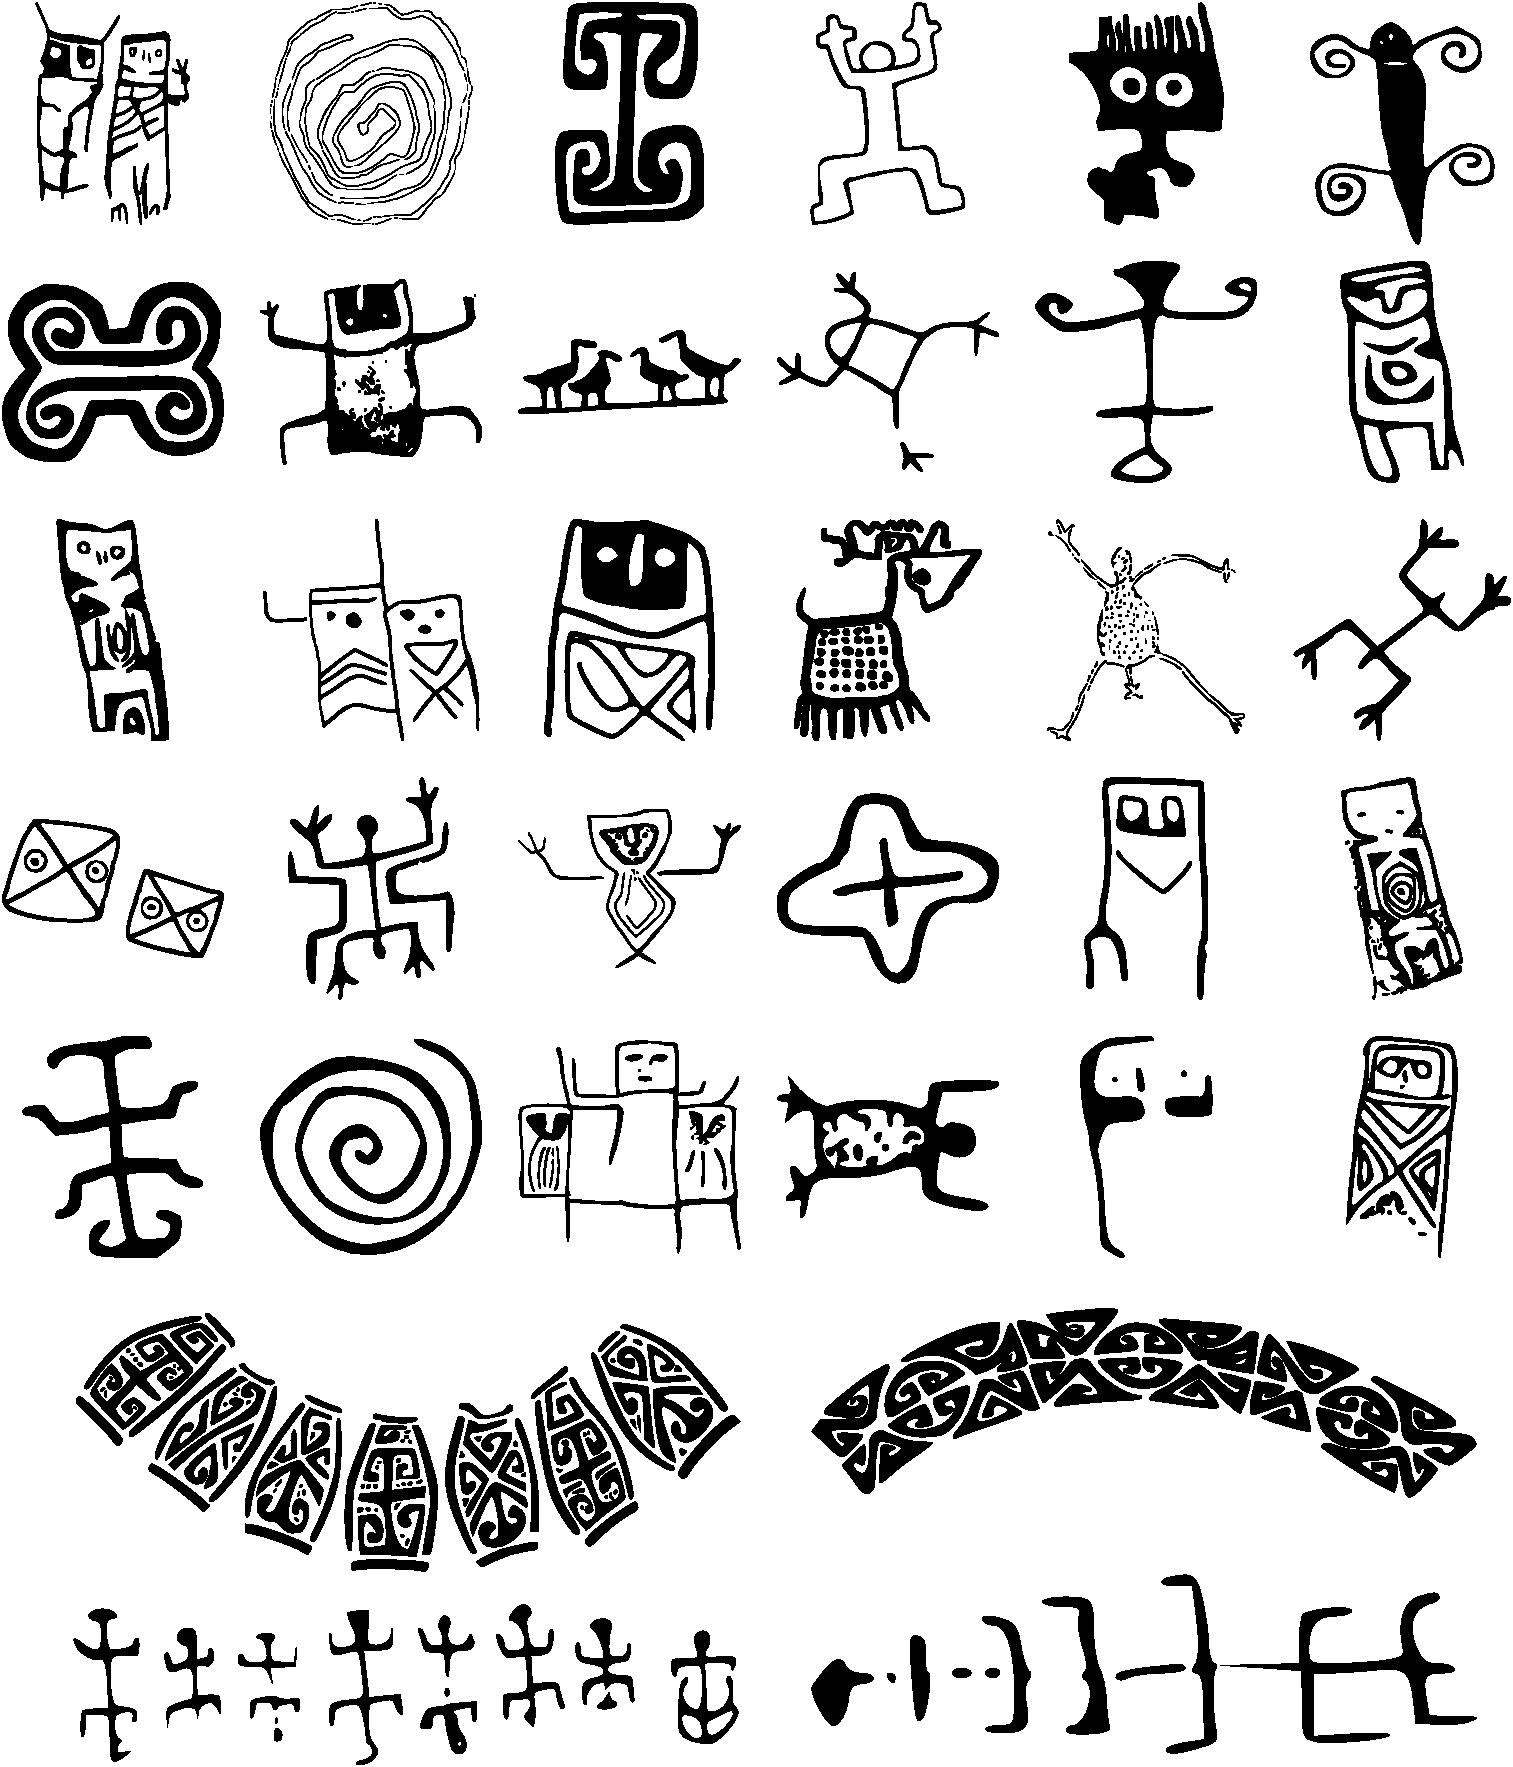
\includegraphics[width=0.8\textwidth]{CALINA/iconografia}
  \end{adjustbox}
  \\
  {\footnotesize Fuente: recopilación del trabajo de \citeA{velandia2019}.}
\end{figure}

\subsection{Selección paleta de colores}

Los tonos bases que se usa en la paleta de colores de la aplicación CALINA, son dos: Vino tinto 
(RGB:119,33,24) y Oro (RGB:241,206,0), haciendo alusión a la bandera del Tolima, el resto de colores son 
seleccionados con base al algoritmo de búsqueda de colores complementarios, esto para dar un buen contraste y 
hacerlo mas atractivo a los menores de edad, escogiendo colores fuera del rango ``tierra'' logrando ser mas 
atractivo para el público objetivo.

\newcommand\palbox[2]{{\sffamily\fboxsep=5pt\relax\fboxrule=1pt\relax\footnotesize%
  \fcolorbox{gray!50}{gray!10}{%
    \stackengine{4pt}{%
      \colorbox[RGB]{#1}{\rule{50pt}{0pt}\rule{0pt}{50pt}}%
    }{%
      \color{black!60}\stackengine{8pt}{\##2}{\scriptsize \saycolors{#1}}{U}{l}{F}{F}{S}%
    }{U}{l}{F}{F}{S}%
  }%
}}
\newcommand\saycolors[1]{\saycolorsaux#1\relax}
\def\saycolorsaux#1 #2 #3\relax{R:#1 G:#2 B:#3}

\begin{figure}[!htb]
\caption{Paleta de colores seleccionada}
\label{img:paletacolores}
\centering
\palbox{119 33 24}{772118}\quad
\palbox{241 206 0}{F1CE00}\quad
\palbox{19 52 237}{1334ED}\quad
\palbox{14 29 31}{0E1D1F}\quad
\palbox{7 90 99}{075A63}
\\ \vspace{4mm}
{\footnotesize Fuente: de elaboración propia}
\end{figure}

\subsection{Diseño GUI de la aplicación CALINA}

A continuación en la figura \ref{img:guicalina}, se muestran un prototipo elaborado para mostrar como se ve 
gráficamente la aplicación CALINA y sus componentes principales.

\begin{figure}[!htb]
\caption{Prototipo GUI CALINA, pantalla principal estudiante}
\label{img:guicalina}
\centering
\begin{adjustbox}{width=15cm}
	\begin{tikzpicture}
	\node[inner sep=0pt] at (0cm,0cm) {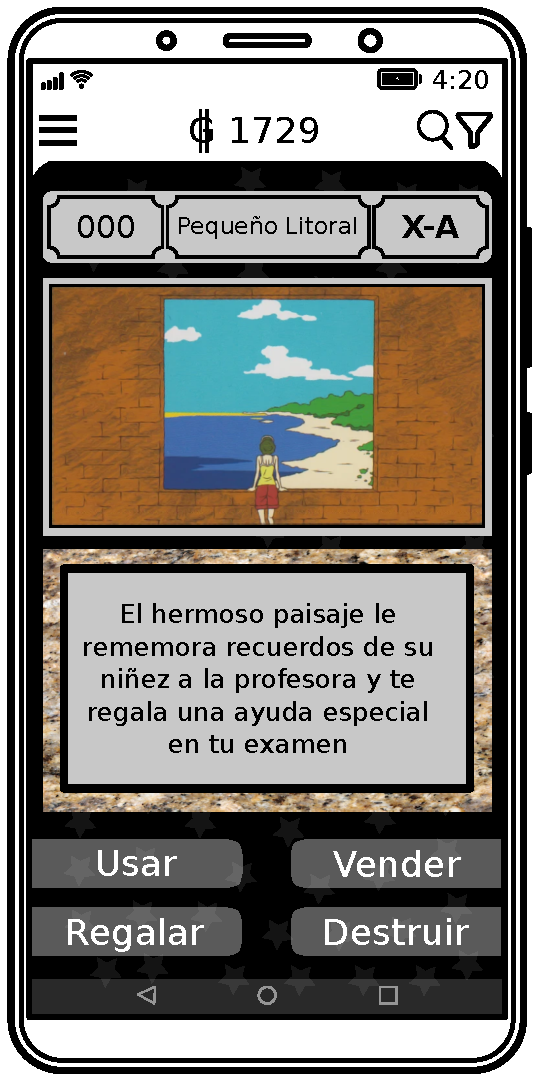
\includegraphics[width=7cm]{prototipos/prototipo1}};
	\draw[red, line width=0.4mm] (-3.05cm, 5cm) rectangle (-2.4cm, 5.65cm) {};
	\draw[red, line width=0.4mm] (-4cm, 5.32cm) -- (-3.05cm, 5.32cm);
	\node[red, anchor=east] at (-4.05cm, 5.32cm) {\textlangle A\textrangle\ Menú de navegación};
	\draw[red, line width=0.4mm] (2.4cm, 5cm) rectangle (2.9cm, 5.65cm) {};
	\draw[red, line width=0.4mm] (2.9cm, 5.32cm) -- (4cm, 5.32cm);
	\node[red, anchor=west] at (4.05cm, 5.32cm) {\textlangle B\textrangle\ Menú de filtro};
	\draw[red, line width=0.4mm] (1.9cm, 5cm) rectangle (2.4cm, 5.65cm) {};
	\draw[red, line width=0.4mm] (2.15cm, 5.65cm) -- (2.15cm, 6.5cm);
	\draw[red, line width=0.4mm] (2.15cm, 6.5cm) -- (4cm, 6.5cm);
	\node[red, anchor=west] at (4.05cm, 6.5cm) {\textlangle C\textrangle\ Menú de búsqueda};
	\draw[red, line width=0.4mm] (-1.4cm, 5cm) rectangle (1cm, 5.65cm) {};
	\draw[red, line width=0.4mm] (-0.2cm, 5.65cm) -- (-0.2cm, 7.5cm);
	\node[red, anchor=south] at (-0.2cm, 7.5cm) {\textlangle D\textrangle\ Indicador divisa virtual};
	\draw[red, line width=0.4mm] (-3.05cm, -3.6cm) rectangle (2.95cm, 4.7cm) {};
	\draw[red, line width=0.4mm] (-4cm, 0.55cm) -- (-3.05cm, 0.55cm);
	\node[red, anchor=east] at (-4.05cm, 0.55cm) {\textlangle E\textrangle\ Zona de las cartas};
	\draw[red, line width=0.4mm] (-3.05cm, -5.5cm) rectangle (2.95cm, -3.7cm) {};
	\draw[red, line width=0.4mm] (-4cm, -4.6cm) -- (-3.05cm, -4.6cm);
	\node[red, anchor=east] at (-4.05cm, -4.6cm) {\textlangle F\textrangle\ Zona de controles};
\end{tikzpicture}

\end{adjustbox}
\\
{\footnotesize Fuente: de elaboración propia}
\end{figure}

\begin{description}
  \item[\textlangle A\textrangle\ Menú de navegación] \hfill \\ Este es el menú desplegable principal de la 
	aplicación CALINA, en este menú el usuario puede ver su perfil, cambiar de curso (por si esta 
	inscrito o es propietario de varios), cambiar algunas opciones de configuración, etc.
  \item[\textlangle B\textrangle\ Menú de filtro] \hfill \\ Este es el menú desplegable sirve para poder 
	filtrar las cartas de acuerdo a su tipo o dificultad.
  \item[\textlangle C\textrangle\ Menú de búsqueda] \hfill \\ Este es el menú desplegable sirve para poder 
	buscar cartas por su nombre o su numeración.
  \item[\textlangle D\textrangle\ Indicador divisa virtual] \hfill \\ En este apartado se puede ver la 
	cantidad de dinero virtual que el estudiante tiene para el curso seleccionado.
  \item[\textlangle E\textrangle\ Zona de cartas] \hfill \\ Zona donde se muestra la cartas de CALINA.
  \item[\textlangle F\textrangle\ Zona de controles] \hfill \\ Zona donde se muestran los controles que pueden 
	ser usados sobre la carta actualmente seleccionada.
\end{description}

\subsection{Arquitectura de la aplicación CALINA}

En el desarrollo de la aplicación CALINA se va a usar la arquitectura MVVM recomendada por google 
(\textit{Model-View-View Model}, \citeA{google2022}), la cual se basa en el principio de separación de 
funciones, con el objetivo de separar la lógica, el manejo de datos, las dependencias y la interfaz gráfica. 
En el caso del software CALINA se van a emplear tres capas: la capa de la UI (\textit{User Interface}), la 
capa de dominio (Casos de uso) y la capa de datos (DAO, \textit{Data Access Object}).

\begin{figure}[ht]
\caption{Arquitectura MVVM aplicación CALINA}
\label{img:arquitectura}
\centering
\begin{tikzpicture}[
		redondeado/.style={draw,align=left,rounded corners=.15cm,inner sep=10pt, minimum width=150pt}
  	]
	\node[redondeado, minimum width=200pt, minimum height=115pt] at (0,7.7) {};
	\node[] at (-1.8,9.1) {\textbf{Capa de la UI}};
	\node[redondeado](UI) at (0,8) {Elementos UI};
	\node[redondeado](estado) at (0,6.5) {Soporte de Estados};

	\node[redondeado](dominio) at (0,4.5) {\textbf{Capa de Dominio}};

	\node[redondeado, minimum width=200pt, minimum height=115pt, fill=mydarkgray] at (0,1.2) {};
	\node[] (temp) at (0,3.4) {};
	\node[text=white] at (-1.8,2.6) {\textbf{Capa de Datos}};
	\node[redondeado, text=white, draw=white] (repositorios) at (0,1.5) {Repositorios};
	\node[redondeado, text=white, draw=white] (datos) at (0,0) {Fuentes de datos};

	\draw[-triangle 90] (UI) edge (estado);
	\draw[-triangle 90] (estado) edge (dominio);
	\draw[-triangle 90] (dominio) edge (repositorios);
	\draw[-triangle 90, white] (temp) edge (repositorios);
	\draw[-triangle 90, white] (repositorios) edge (datos);
\end{tikzpicture}

\\
{\footnotesize Fuente: Guía de arquitectura de apps, \citeA{google2022}}
\end{figure}

Para la implementación del software se usa lenguaje \textit{Kotlin} como base, usando \textit{Jetpack Compose} 
para el desarrollo de la interfaz gráfica, y \textit{Room} para el manejo de la base de datos.

\subsection{Modelo de datos internos CALINA}

La aplicación CALINA usa una única tabla para gestionar la persistencia de datos, implementada sobre el 
sistema de gestión de base de datos relacional \textit{SQLite}.

\begin{figure}[ht]
\caption{Diagrama ER (Entidad Relación), base de datos interna}
\label{img:diagramaER}
\centering
\begin{tikzpicture}[
		redondeado/.style={draw,align=left,rounded corners=.15cm,inner sep=10pt, minimum width=150pt}
  	]
	
	\node[redondeado, minimum width=200pt, minimum height=370pt, fill=mygray, draw=none, anchor=north west] 
		at (-3.4,9.4) {};
	\node[redondeado, minimum width=200pt, minimum height=370pt, fill=white, anchor=north west] 
		at (-3.5,9.5) {};
	
	\node[] at (-1.8,9.8) {\textbf{CALINA.Card}};

	\node[anchor=west] at (-3,9)  {\faKey\hspace{0.2em} imei\_card};
	\node[anchor=west] at (1.7,9) {string};
	\node[anchor=west] at (-3,8.5)  {\faKey\hspace{0.2em} imei\_maker};
	\node[anchor=west] at (1.7,8.5) {string};
	\draw (-3.2,8) -- (3.2,8);
	\node[anchor=west] at (-3,7.5)  {title};
	\node[anchor=west] at (1.7,7.5) {string};
	\node[anchor=west] at (-3,7)  {description};
	\node[anchor=west] at (1.7,7) {string};
	\node[anchor=west] at (-3,6.5)  {type};
	\node[anchor=west] at (1.7,6.5) {char};
	\node[anchor=west] at (-3,6)  {difficulty};
	\node[anchor=west] at (1.7,6) {char};
	\node[anchor=west] at (-3,5.5)  {number};
	\node[anchor=west] at (1.7,5.5) {int};
	\node[anchor=west] at (-3,5)  {imei\_owner};
	\node[anchor=west] at (1.7,5) {string};
	\node[anchor=west] at (-3,4.5)  {image};
	\node[anchor=west] at (1.7,4.5) {string};
	\node[anchor=west] at (-3,4)  {trigger=``''};
	\node[anchor=west] at (1.7,4) {string};
	\node[anchor=west] at (-3,3.5)  {state='N'};
	\node[anchor=west] at (1.7,3.5) {char};
	\node[anchor=west] at (-3,3)  {versionCALINA};
	\node[anchor=west] at (1.7,3) {string};
	\node[anchor=west] at (-3,2.5)  {date\_create=null};
	\node[anchor=west] at (1.7,2.5) {date};
	\node[anchor=west] at (-3,2)  {date\_expire=null};
	\node[anchor=west] at (1.7,2) {date};
	\node[anchor=west] at (-3,1.5)  {scope=-1};
	\node[anchor=west] at (1.7,1.5) {int};
	\node[anchor=west] at (-3,1)  {isTransfer=true};
	\node[anchor=west] at (1.7,1) {bool};
	\node[anchor=west] at (-3,0.5)  {isCloneable=false};
	\node[anchor=west] at (1.7,0.5) {bool};
	\node[anchor=west] at (-3,0)  {isEdit=false};
	\node[anchor=west] at (1.7,0) {bool};
	\node[anchor=west] at (-3,-0.5)  {cash=0};
	\node[anchor=west] at (1.7,-0.5) {int};
	\node[anchor=west] at (-3,-1)  {cash\_symbol='¢'};
	\node[anchor=west] at (1.7,-1) {char};
	\node[anchor=west] at (-3,-1.5)  {isSelect=false};
	\node[anchor=west] at (1.7,-1.5) {bool};
	\node[anchor=west] at (-3,-2)  {isSecondary=false};
	\node[anchor=west] at (1.7,-2) {bool};
	\node[anchor=west] at (-3,-2.5)  {levels=``''};
	\node[anchor=west] at (1.7,-2.5) {string};
	\node[anchor=west] at (-3,-3)  {level=``''};
	\node[anchor=west] at (1.7,-3) {string};

\end{tikzpicture}

\\
{\footnotesize Fuente: de elaboración propia}
\end{figure}

